% Options for packages loaded elsewhere
\PassOptionsToPackage{unicode}{hyperref}
\PassOptionsToPackage{hyphens}{url}
%
\documentclass[
]{article}
\usepackage{amsmath,amssymb}
\usepackage{lmodern}
\usepackage{ifxetex,ifluatex}
\ifnum 0\ifxetex 1\fi\ifluatex 1\fi=0 % if pdftex
  \usepackage[T1]{fontenc}
  \usepackage[utf8]{inputenc}
  \usepackage{textcomp} % provide euro and other symbols
\else % if luatex or xetex
  \usepackage{unicode-math}
  \defaultfontfeatures{Scale=MatchLowercase}
  \defaultfontfeatures[\rmfamily]{Ligatures=TeX,Scale=1}
\fi
% Use upquote if available, for straight quotes in verbatim environments
\IfFileExists{upquote.sty}{\usepackage{upquote}}{}
\IfFileExists{microtype.sty}{% use microtype if available
  \usepackage[]{microtype}
  \UseMicrotypeSet[protrusion]{basicmath} % disable protrusion for tt fonts
}{}
\makeatletter
\@ifundefined{KOMAClassName}{% if non-KOMA class
  \IfFileExists{parskip.sty}{%
    \usepackage{parskip}
  }{% else
    \setlength{\parindent}{0pt}
    \setlength{\parskip}{6pt plus 2pt minus 1pt}}
}{% if KOMA class
  \KOMAoptions{parskip=half}}
\makeatother
\usepackage{xcolor}
\IfFileExists{xurl.sty}{\usepackage{xurl}}{} % add URL line breaks if available
\IfFileExists{bookmark.sty}{\usepackage{bookmark}}{\usepackage{hyperref}}
\hypersetup{
  pdftitle={LOO\_MRP Simulation Experiments Document},
  pdfauthor={Swen Kuh},
  hidelinks,
  pdfcreator={LaTeX via pandoc}}
\urlstyle{same} % disable monospaced font for URLs
\usepackage[margin=1in]{geometry}
\usepackage{color}
\usepackage{fancyvrb}
\newcommand{\VerbBar}{|}
\newcommand{\VERB}{\Verb[commandchars=\\\{\}]}
\DefineVerbatimEnvironment{Highlighting}{Verbatim}{commandchars=\\\{\}}
% Add ',fontsize=\small' for more characters per line
\usepackage{framed}
\definecolor{shadecolor}{RGB}{248,248,248}
\newenvironment{Shaded}{\begin{snugshade}}{\end{snugshade}}
\newcommand{\AlertTok}[1]{\textcolor[rgb]{0.94,0.16,0.16}{#1}}
\newcommand{\AnnotationTok}[1]{\textcolor[rgb]{0.56,0.35,0.01}{\textbf{\textit{#1}}}}
\newcommand{\AttributeTok}[1]{\textcolor[rgb]{0.77,0.63,0.00}{#1}}
\newcommand{\BaseNTok}[1]{\textcolor[rgb]{0.00,0.00,0.81}{#1}}
\newcommand{\BuiltInTok}[1]{#1}
\newcommand{\CharTok}[1]{\textcolor[rgb]{0.31,0.60,0.02}{#1}}
\newcommand{\CommentTok}[1]{\textcolor[rgb]{0.56,0.35,0.01}{\textit{#1}}}
\newcommand{\CommentVarTok}[1]{\textcolor[rgb]{0.56,0.35,0.01}{\textbf{\textit{#1}}}}
\newcommand{\ConstantTok}[1]{\textcolor[rgb]{0.00,0.00,0.00}{#1}}
\newcommand{\ControlFlowTok}[1]{\textcolor[rgb]{0.13,0.29,0.53}{\textbf{#1}}}
\newcommand{\DataTypeTok}[1]{\textcolor[rgb]{0.13,0.29,0.53}{#1}}
\newcommand{\DecValTok}[1]{\textcolor[rgb]{0.00,0.00,0.81}{#1}}
\newcommand{\DocumentationTok}[1]{\textcolor[rgb]{0.56,0.35,0.01}{\textbf{\textit{#1}}}}
\newcommand{\ErrorTok}[1]{\textcolor[rgb]{0.64,0.00,0.00}{\textbf{#1}}}
\newcommand{\ExtensionTok}[1]{#1}
\newcommand{\FloatTok}[1]{\textcolor[rgb]{0.00,0.00,0.81}{#1}}
\newcommand{\FunctionTok}[1]{\textcolor[rgb]{0.00,0.00,0.00}{#1}}
\newcommand{\ImportTok}[1]{#1}
\newcommand{\InformationTok}[1]{\textcolor[rgb]{0.56,0.35,0.01}{\textbf{\textit{#1}}}}
\newcommand{\KeywordTok}[1]{\textcolor[rgb]{0.13,0.29,0.53}{\textbf{#1}}}
\newcommand{\NormalTok}[1]{#1}
\newcommand{\OperatorTok}[1]{\textcolor[rgb]{0.81,0.36,0.00}{\textbf{#1}}}
\newcommand{\OtherTok}[1]{\textcolor[rgb]{0.56,0.35,0.01}{#1}}
\newcommand{\PreprocessorTok}[1]{\textcolor[rgb]{0.56,0.35,0.01}{\textit{#1}}}
\newcommand{\RegionMarkerTok}[1]{#1}
\newcommand{\SpecialCharTok}[1]{\textcolor[rgb]{0.00,0.00,0.00}{#1}}
\newcommand{\SpecialStringTok}[1]{\textcolor[rgb]{0.31,0.60,0.02}{#1}}
\newcommand{\StringTok}[1]{\textcolor[rgb]{0.31,0.60,0.02}{#1}}
\newcommand{\VariableTok}[1]{\textcolor[rgb]{0.00,0.00,0.00}{#1}}
\newcommand{\VerbatimStringTok}[1]{\textcolor[rgb]{0.31,0.60,0.02}{#1}}
\newcommand{\WarningTok}[1]{\textcolor[rgb]{0.56,0.35,0.01}{\textbf{\textit{#1}}}}
\usepackage{graphicx}
\makeatletter
\def\maxwidth{\ifdim\Gin@nat@width>\linewidth\linewidth\else\Gin@nat@width\fi}
\def\maxheight{\ifdim\Gin@nat@height>\textheight\textheight\else\Gin@nat@height\fi}
\makeatother
% Scale images if necessary, so that they will not overflow the page
% margins by default, and it is still possible to overwrite the defaults
% using explicit options in \includegraphics[width, height, ...]{}
\setkeys{Gin}{width=\maxwidth,height=\maxheight,keepaspectratio}
% Set default figure placement to htbp
\makeatletter
\def\fps@figure{htbp}
\makeatother
\setlength{\emergencystretch}{3em} % prevent overfull lines
\providecommand{\tightlist}{%
  \setlength{\itemsep}{0pt}\setlength{\parskip}{0pt}}
\setcounter{secnumdepth}{-\maxdimen} % remove section numbering
\ifluatex
  \usepackage{selnolig}  % disable illegal ligatures
\fi

\title{LOO\_MRP Simulation Experiments Document}
\author{Swen Kuh}
\date{22/11/2021}

\begin{document}
\maketitle

\hypertarget{simulation-2}{%
\section{Simulation 2}\label{simulation-2}}

\hypertarget{super-population-approach}{%
\subsection{Super-population approach}\label{super-population-approach}}

Now, we have the above code in the for-loop, generating different
population and samples from that population each time.

In addition, we also introduced `\texttt{LOOP}' -- a weighted loo
estimate by weighting using the MRP estimates.

\hypertarget{using-loo}{%
\subsubsection{\texorpdfstring{\textbf{Using
LOO}:}{Using LOO:}}\label{using-loo}}

This time with a super-population approach, the trend is a bit clearer
to what we have expected. Models with \(X_2\) and \(X_4\) (models \#9,
\#12, \#14) are slightly preferred when compared to the full model
(model \#15) with all the variables \(X_1, X_2, X_3, X_4\). That means
with the variables that are strongly predictive of the outcome and
survey response, we do not need the variables that are weakly
predictive. The results are the same whether we use \texttt{loo},
\texttt{wtd\_loo}, or \texttt{LOOP}.

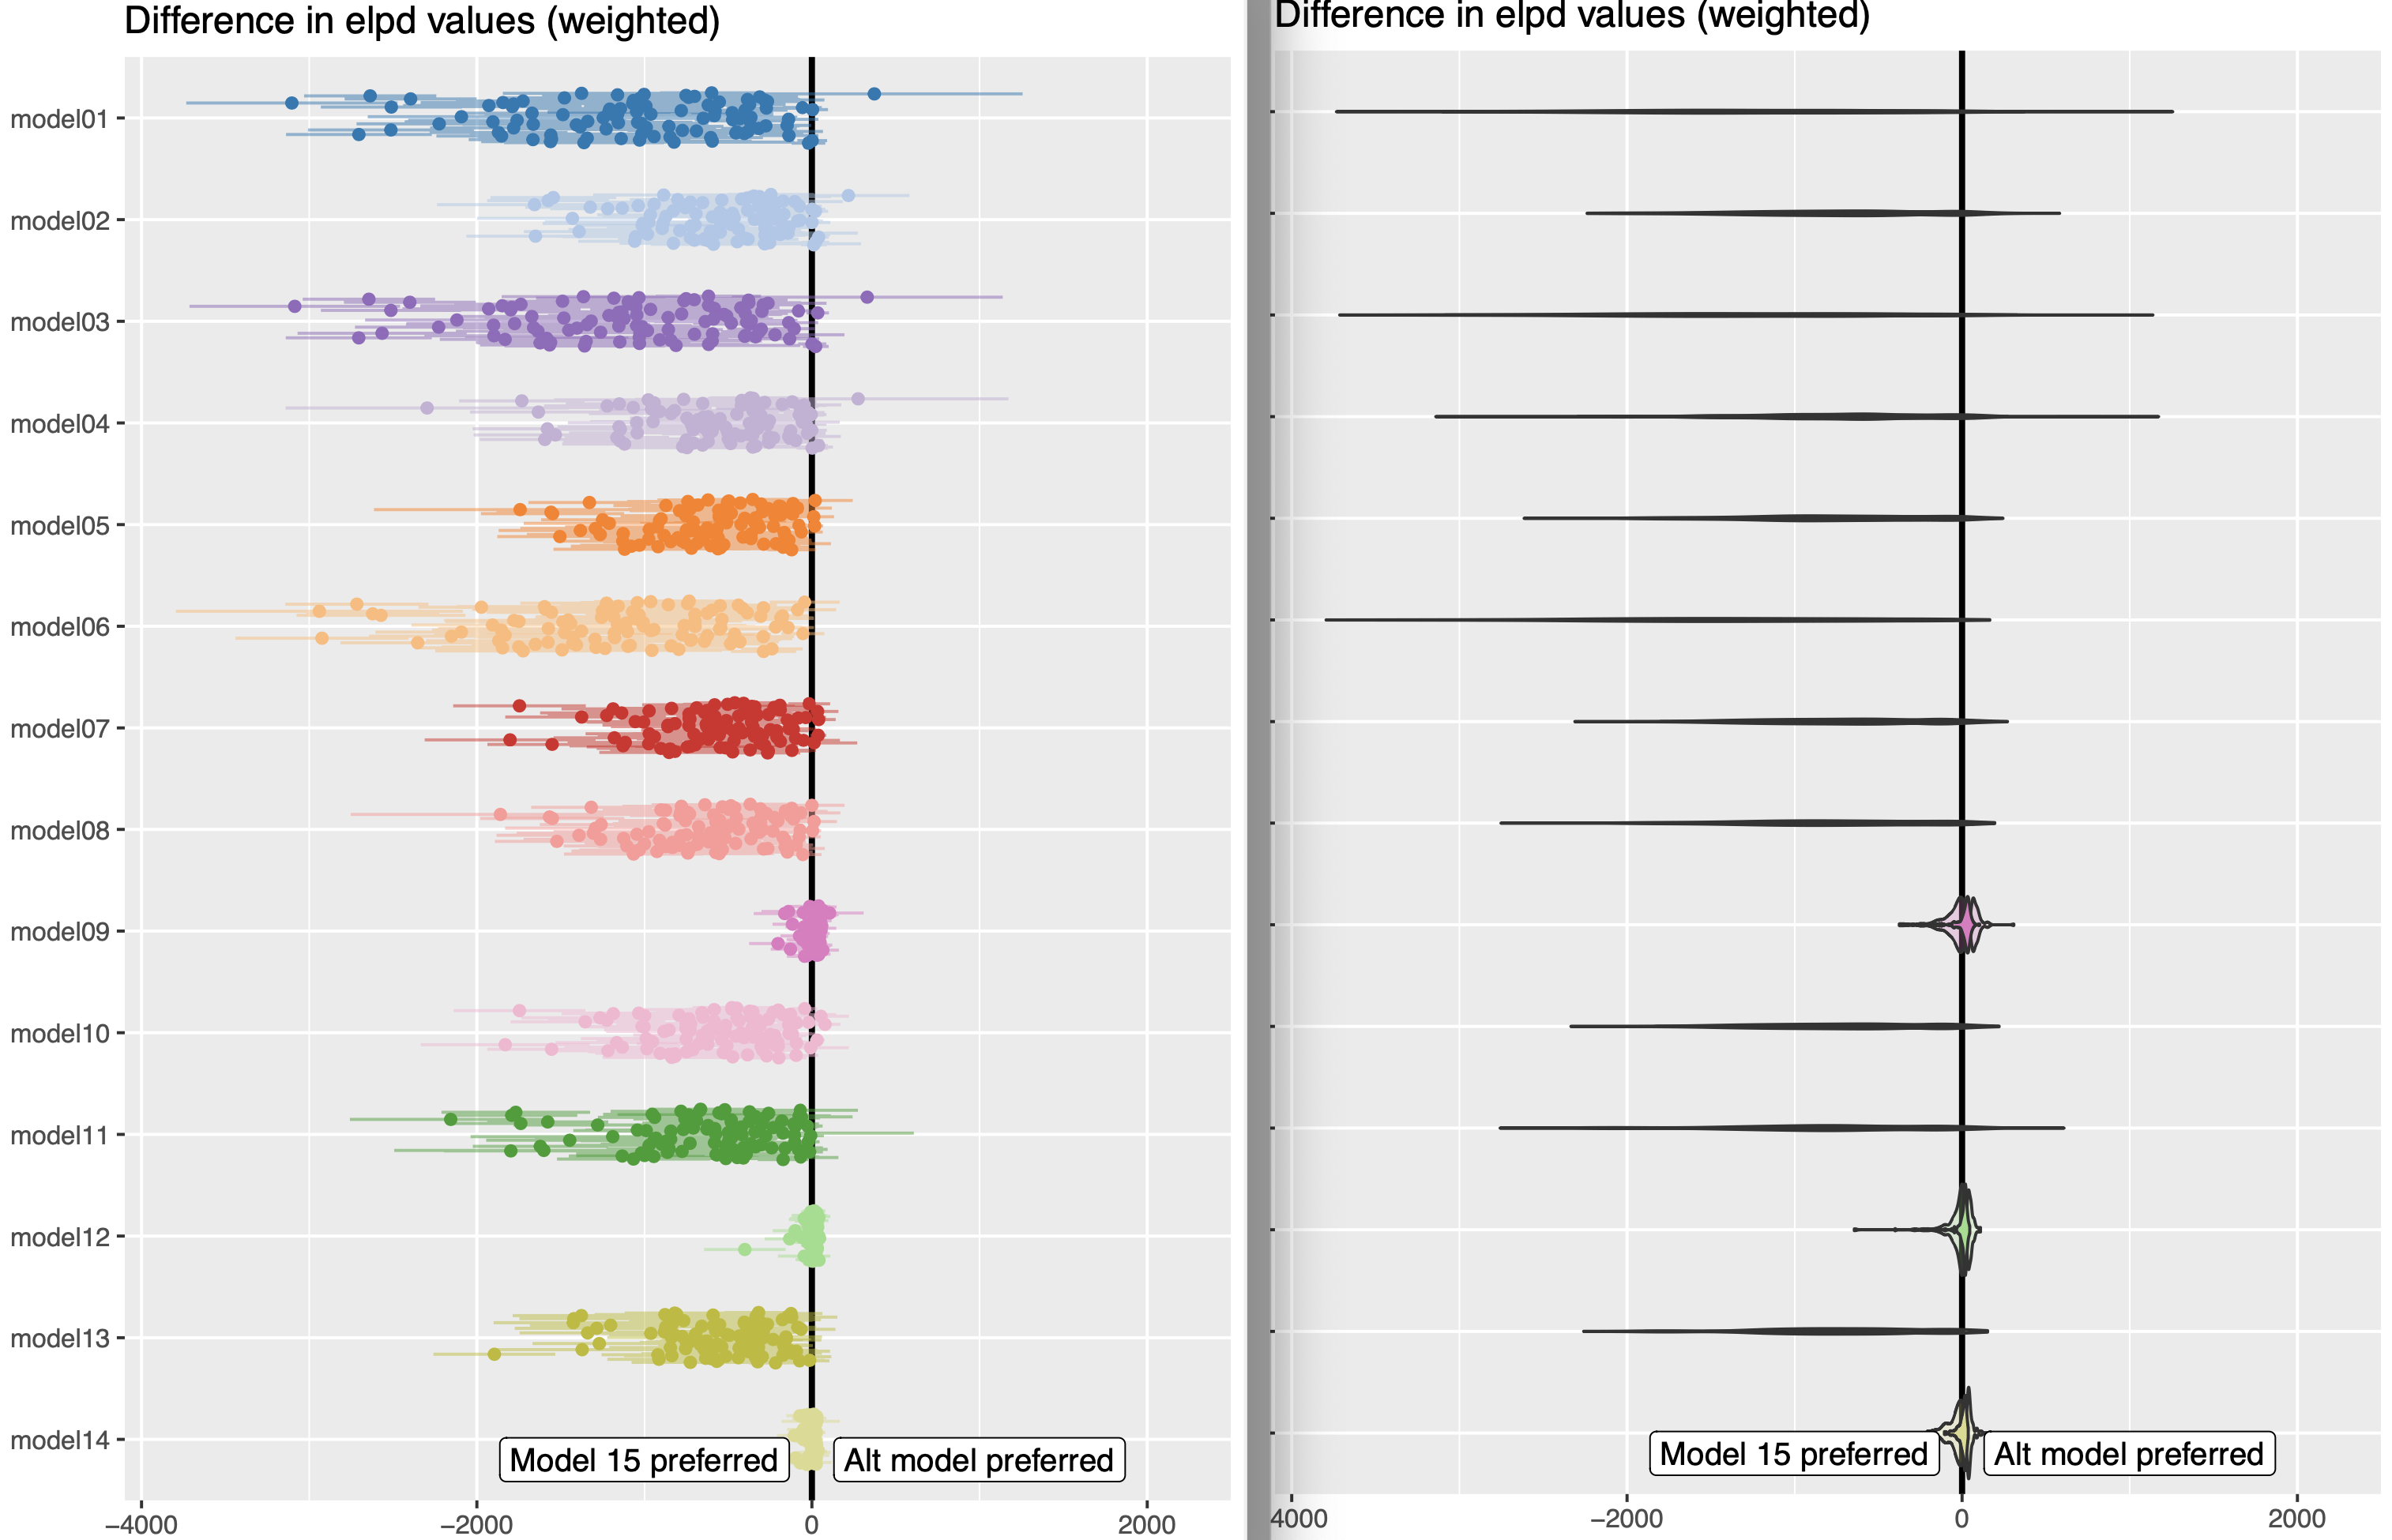
\includegraphics{images/image-1.png}
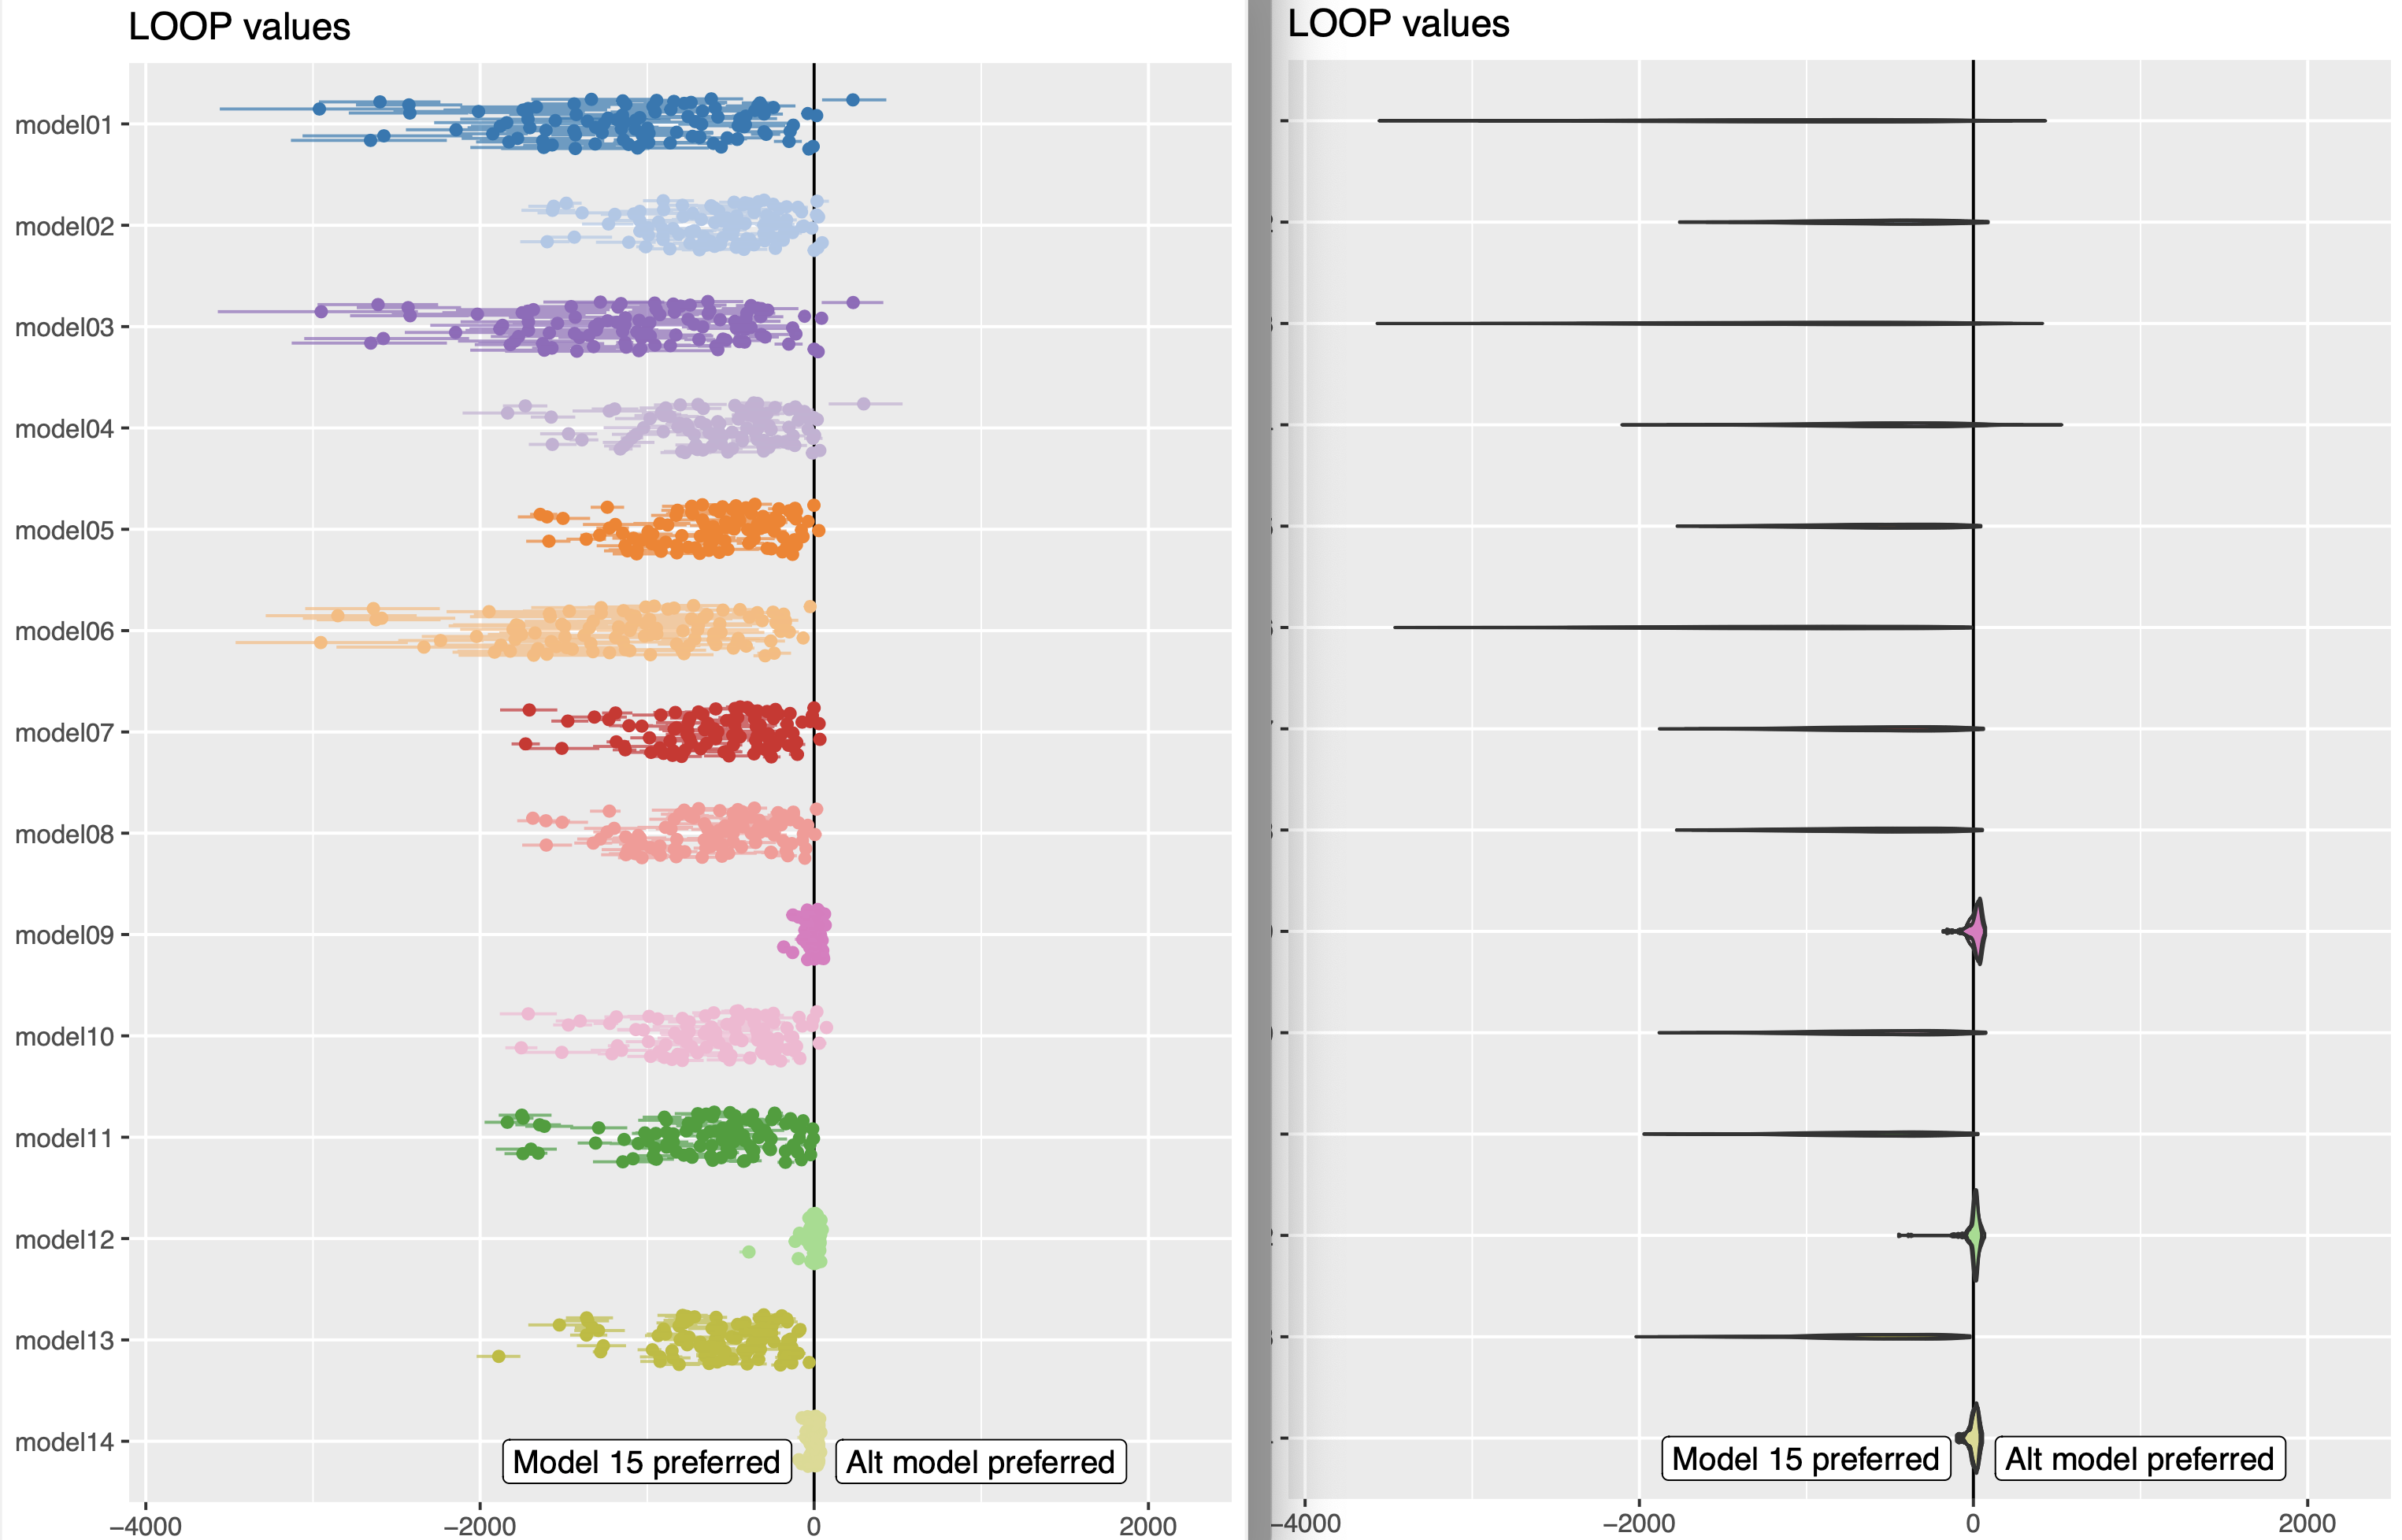
\includegraphics{images/image-2.png}
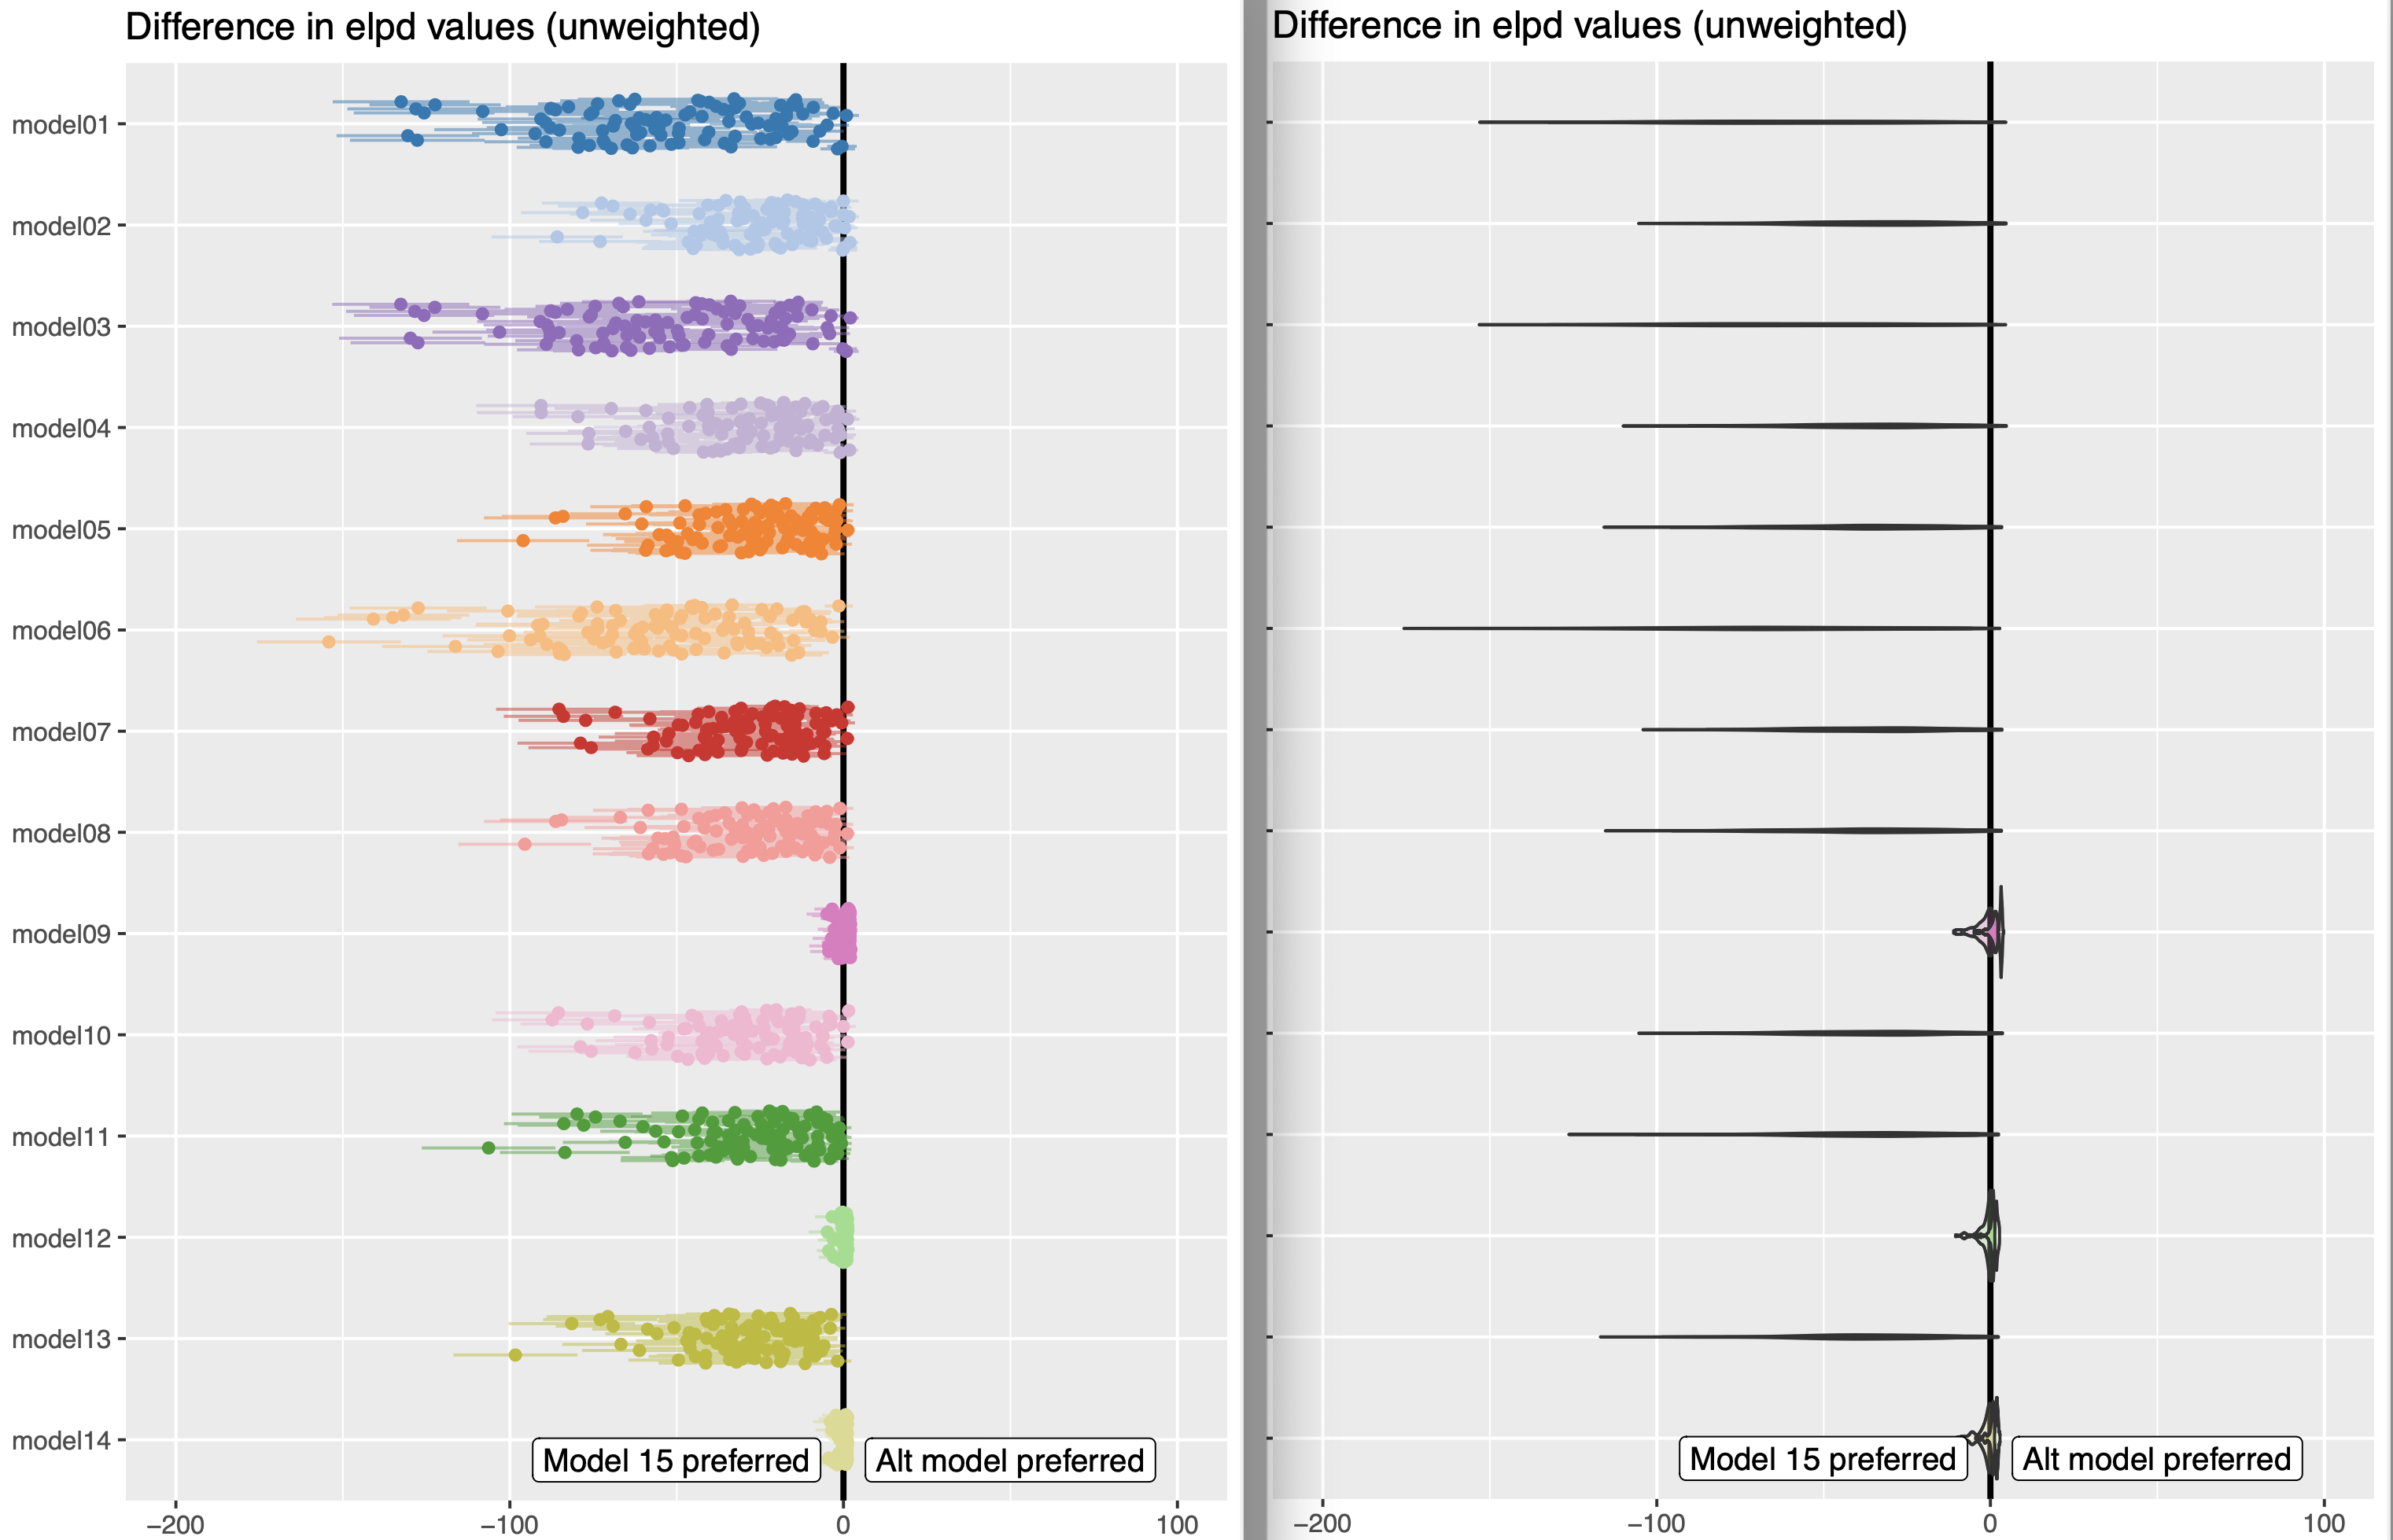
\includegraphics{images/image-3.png}

\hypertarget{using-mrp-estimates}{%
\subsubsection{\texorpdfstring{\textbf{Using MRP
estimates}:}{Using MRP estimates:}}\label{using-mrp-estimates}}

When we assess the model performance based on its predictive power of
the (binary) outcome, we can see that any model with \(X_4\) in it
(models \#4, \#7, \#9, \#10, \#11, \#12, \#13, \#14, \#15) has less
uncertainty in the biases.

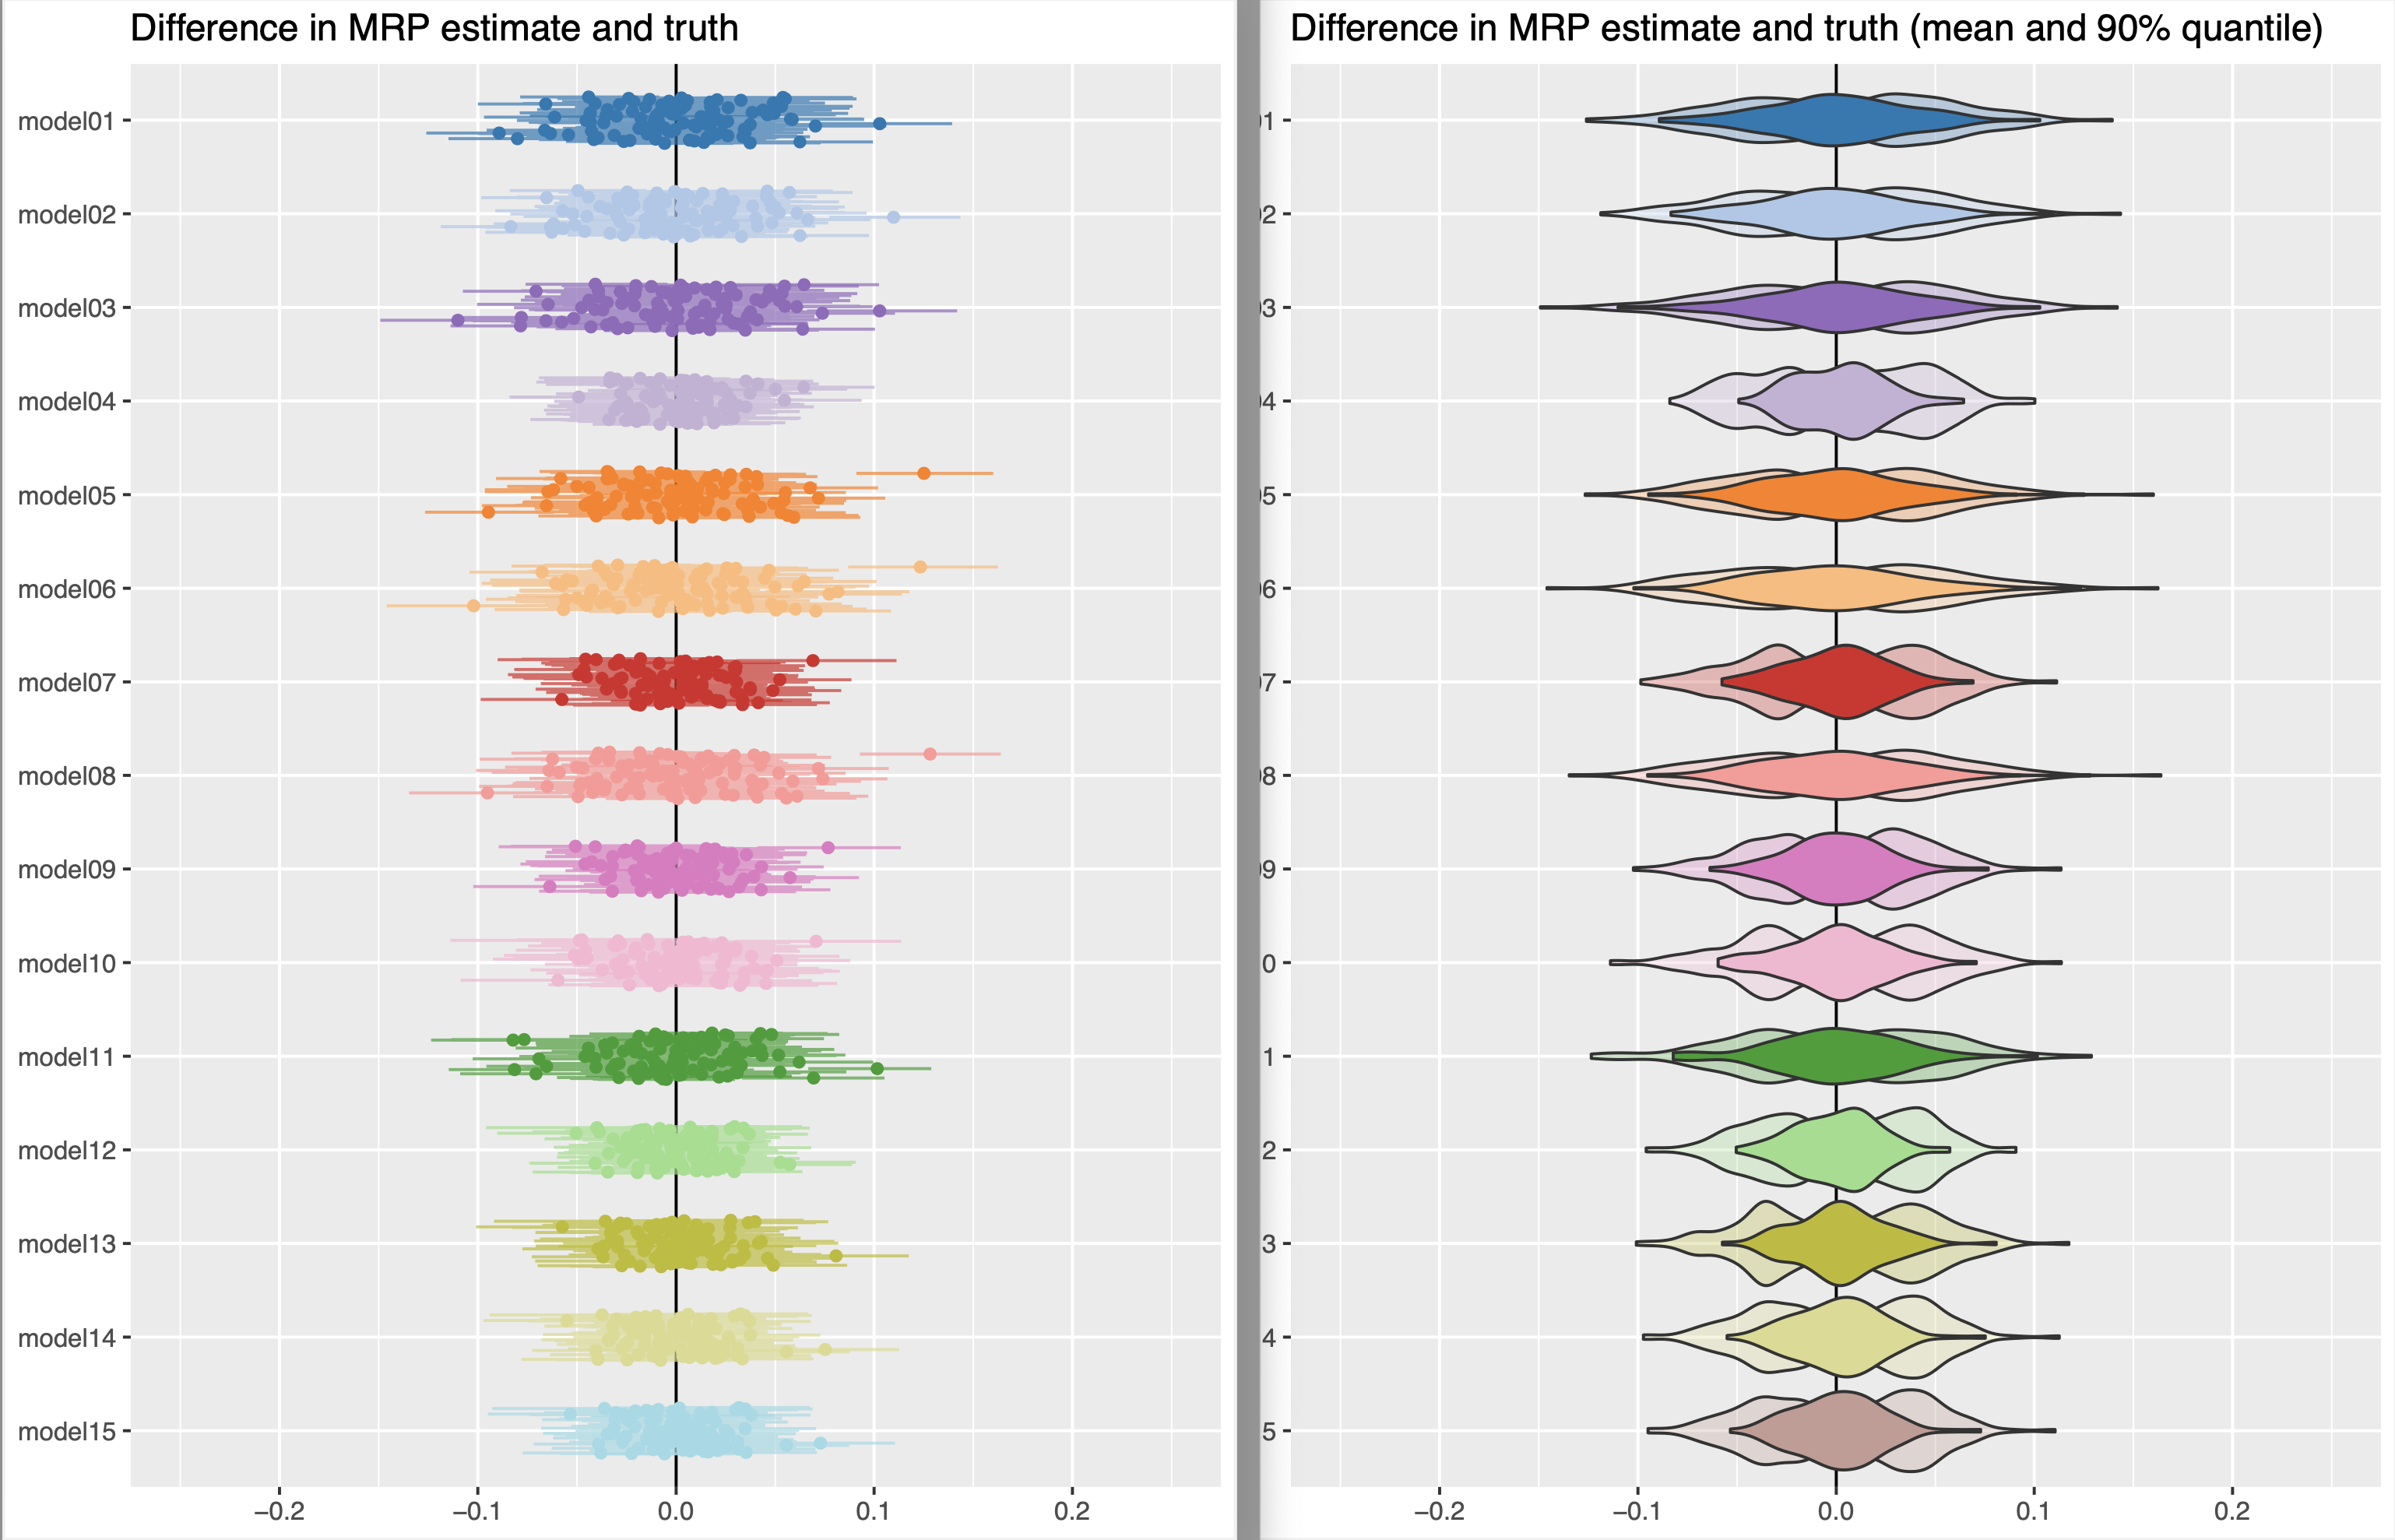
\includegraphics{images/image.png}

\begin{quote}
LOO suggests equivalence of any models with \(X_2 + X_4\)
\(\leftrightarrow\) \newline MRP estimates: models with \(X_4\) ?
\end{quote}

\hypertarget{simulation-2b}{%
\section{Simulation 2b}\label{simulation-2b}}

\hypertarget{super-population-approach-with-continuous-covariates}{%
\subsection{Super-population approach with continuous
covariates}\label{super-population-approach-with-continuous-covariates}}

Now instead of generating the outcome using discrete covariates, we
generate the outcome variable using the continuous covariates so that it
has a stronger relationship with the outcome.

We have also sampled part of the data using `brute-force', by making
sure we sample at least one from each level of covariate, so that we
don't run into issue when calculating the weights.

\begin{Shaded}
\begin{Highlighting}[]
\DocumentationTok{\#\# generating 5 continuous predictors/covariates}
\NormalTok{N }\OtherTok{=} \DecValTok{10000}

\DocumentationTok{\#\# generating a binary outcome }
\CommentTok{\# weakly predictive {-} 0.1 (sd), strongly predictive {-} 1 (sd)}
\FunctionTok{set.seed}\NormalTok{(}\DecValTok{65438}\NormalTok{)}
\NormalTok{pn }\OtherTok{=} \DecValTok{100} \CommentTok{\# number of population}
\NormalTok{seed }\OtherTok{=} \FunctionTok{round}\NormalTok{(}\FunctionTok{runif}\NormalTok{(pn, }\AttributeTok{min=}\DecValTok{10}\NormalTok{, }\AttributeTok{max=}\DecValTok{100000}\NormalTok{),}\DecValTok{0}\NormalTok{) }\CommentTok{\# fixed seed number}

\ControlFlowTok{for}\NormalTok{ (i }\ControlFlowTok{in} \DecValTok{1}\SpecialCharTok{:}\NormalTok{ITE)\{}
 \FunctionTok{set.seed}\NormalTok{(seed[i])}
\NormalTok{  popn\_data }\OtherTok{\textless{}{-}} \FunctionTok{data.frame}\NormalTok{(}\AttributeTok{X1\_cont =} \FunctionTok{rnorm}\NormalTok{(N, }\DecValTok{0}\NormalTok{, }\DecValTok{2}\NormalTok{), }
                          \AttributeTok{X2\_cont =} \FunctionTok{rnorm}\NormalTok{(N, }\DecValTok{0}\NormalTok{, }\DecValTok{2}\NormalTok{),}
                          \AttributeTok{X3\_cont =} \FunctionTok{rnorm}\NormalTok{(N, }\DecValTok{0}\NormalTok{, }\DecValTok{2}\NormalTok{), }
                          \AttributeTok{X4\_cont =} \FunctionTok{rnorm}\NormalTok{(N, }\DecValTok{0}\NormalTok{, }\DecValTok{2}\NormalTok{))}
  
  
\NormalTok{  wkly1 }\OtherTok{=} \FloatTok{0.1}
\NormalTok{  strg1 }\OtherTok{=} \DecValTok{1}
  
  \DocumentationTok{\#\# generating continuous and binary outcome}
\NormalTok{  popn\_data}\SpecialCharTok{$}\NormalTok{outcome }\OtherTok{\textless{}{-}} \FunctionTok{inv\_logit\_scaled}\NormalTok{(wkly1}\SpecialCharTok{*}\NormalTok{popn\_data}\SpecialCharTok{$}\NormalTok{X1\_cont }\SpecialCharTok{+}
\NormalTok{                                          strg1}\SpecialCharTok{*}\NormalTok{popn\_data}\SpecialCharTok{$}\NormalTok{X2\_cont }\SpecialCharTok{+}
\NormalTok{                                          wkly1}\SpecialCharTok{*}\NormalTok{popn\_data}\SpecialCharTok{$}\NormalTok{X3\_cont }\SpecialCharTok{+}
\NormalTok{                                          strg1}\SpecialCharTok{*}\NormalTok{popn\_data}\SpecialCharTok{$}\NormalTok{X4\_cont)}
\NormalTok{  popn\_data}\SpecialCharTok{$}\NormalTok{bin\_value }\OtherTok{\textless{}{-}} \FunctionTok{rbinom}\NormalTok{(N,}\DecValTok{1}\NormalTok{,popn\_data}\SpecialCharTok{$}\NormalTok{outcome)}
  
  
  \DocumentationTok{\#\# generate inclusion prob. for each individual}
  \CommentTok{\# weakly predictive {-} 0.1 (sd), strongly predictive {-} 1 (sd)}
\NormalTok{  wkly2 }\OtherTok{=} \FloatTok{0.1}
\NormalTok{  strg2 }\OtherTok{=} \DecValTok{1}
\NormalTok{  popn\_data}\SpecialCharTok{$}\NormalTok{incl\_prob }\OtherTok{\textless{}{-}} \FunctionTok{inv\_logit\_scaled}\NormalTok{(wkly2}\SpecialCharTok{*}\NormalTok{popn\_data}\SpecialCharTok{$}\NormalTok{X1\_cont }\SpecialCharTok{+} 
\NormalTok{                                            wkly2}\SpecialCharTok{*}\NormalTok{popn\_data}\SpecialCharTok{$}\NormalTok{X2\_cont }\SpecialCharTok{+} 
\NormalTok{                                            strg2}\SpecialCharTok{*}\NormalTok{popn\_data}\SpecialCharTok{$}\NormalTok{X3\_cont }\SpecialCharTok{+}
\NormalTok{                                            strg2}\SpecialCharTok{*}\NormalTok{popn\_data}\SpecialCharTok{$}\NormalTok{X4\_cont)}
\end{Highlighting}
\end{Shaded}

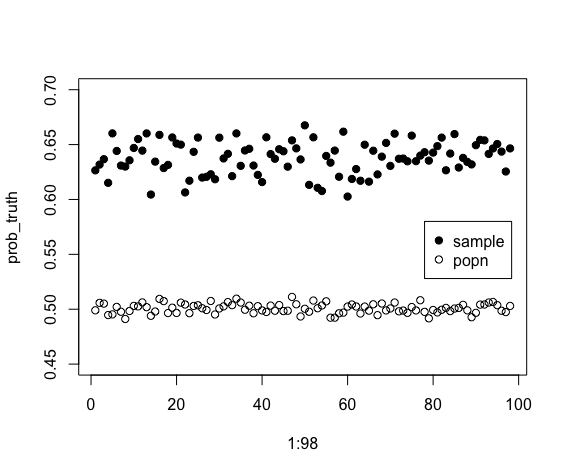
\includegraphics[width=3.125in,height=\textheight]{images/3b/probTruth.png}

If we look at the unweighted elpd LOO values, models \#9,12,14 (the ones
with both \(X_2\) and \(X_4\)) are preferred, followed by the models
with \(X_2\) in it, then with \(X_4\), and finally the ones with \(X_1\)
and \(X_3\) only) are distinctively `un-preferred'. But we have higher
precision for the the LOO estimates using just \(X_4\) only.

If we weigh the elpd values, the distinctions between using \(X_4\) and
\(X_2\) only models decreases.

We see similar conclusion by looking at the LOOP values (adjust using
MRP).

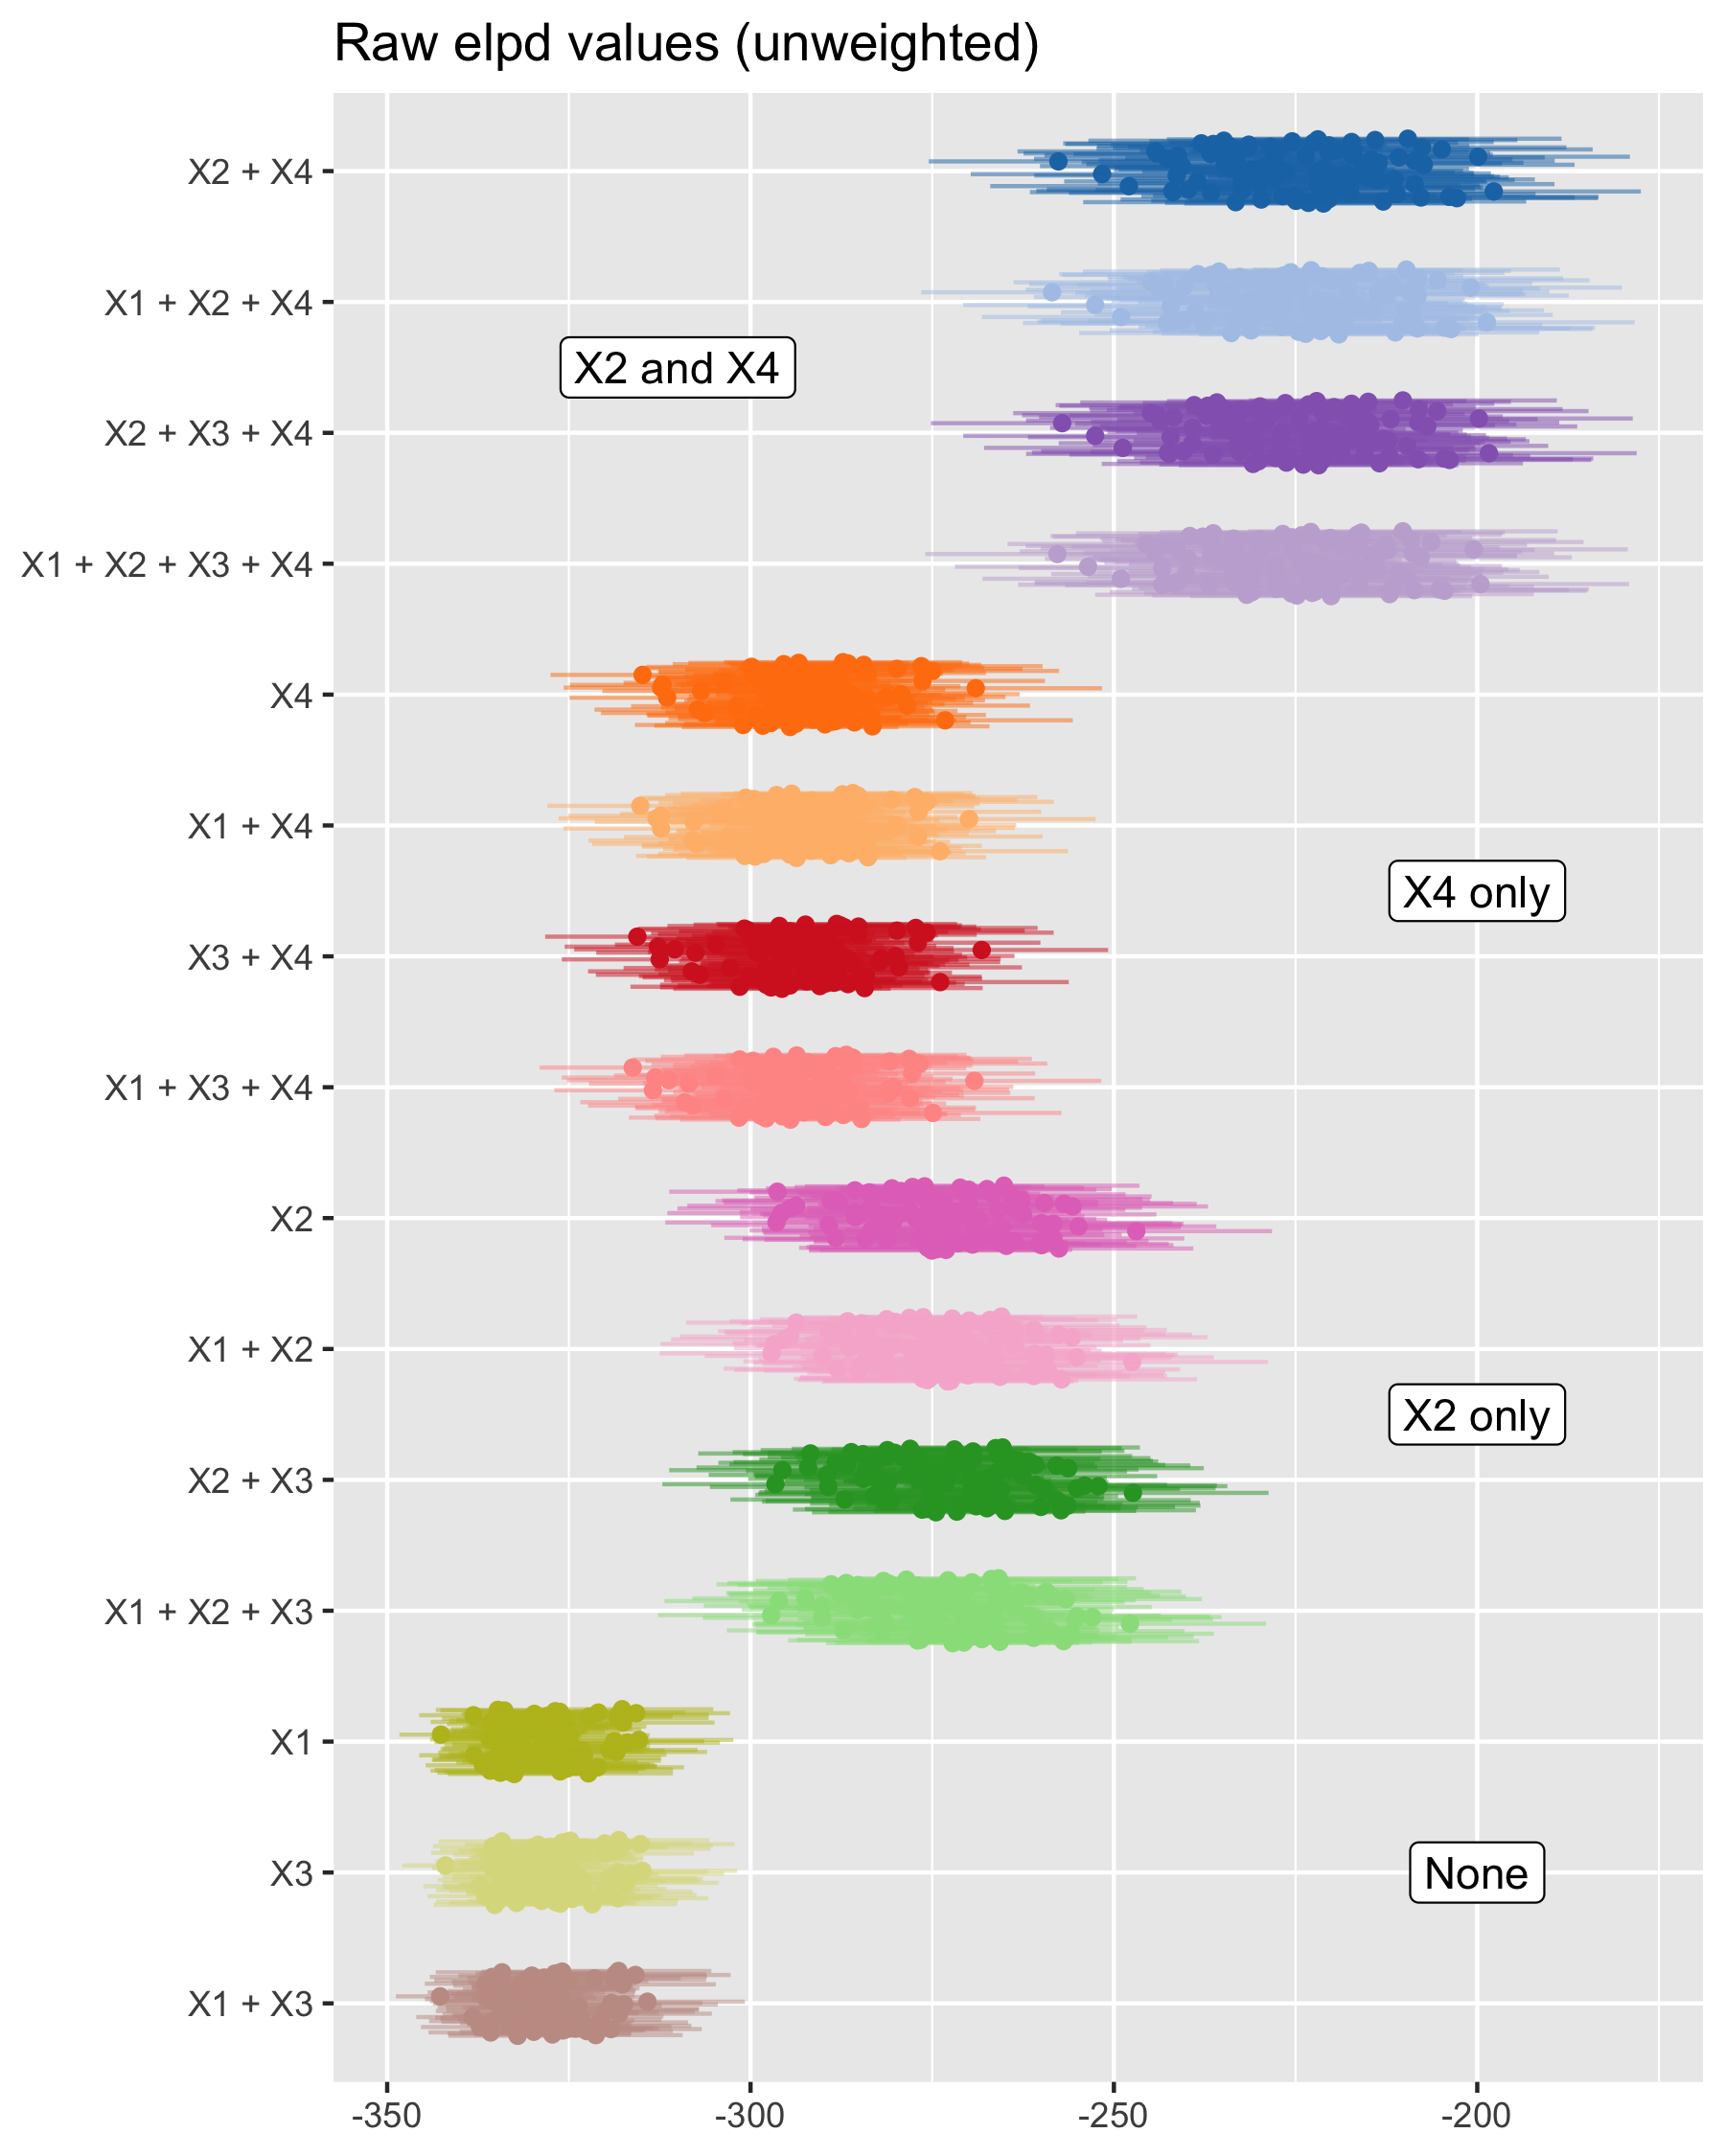
\includegraphics[width=4.6875in,height=\textheight]{images/3b/plot_loo_raw_unwtd.png}
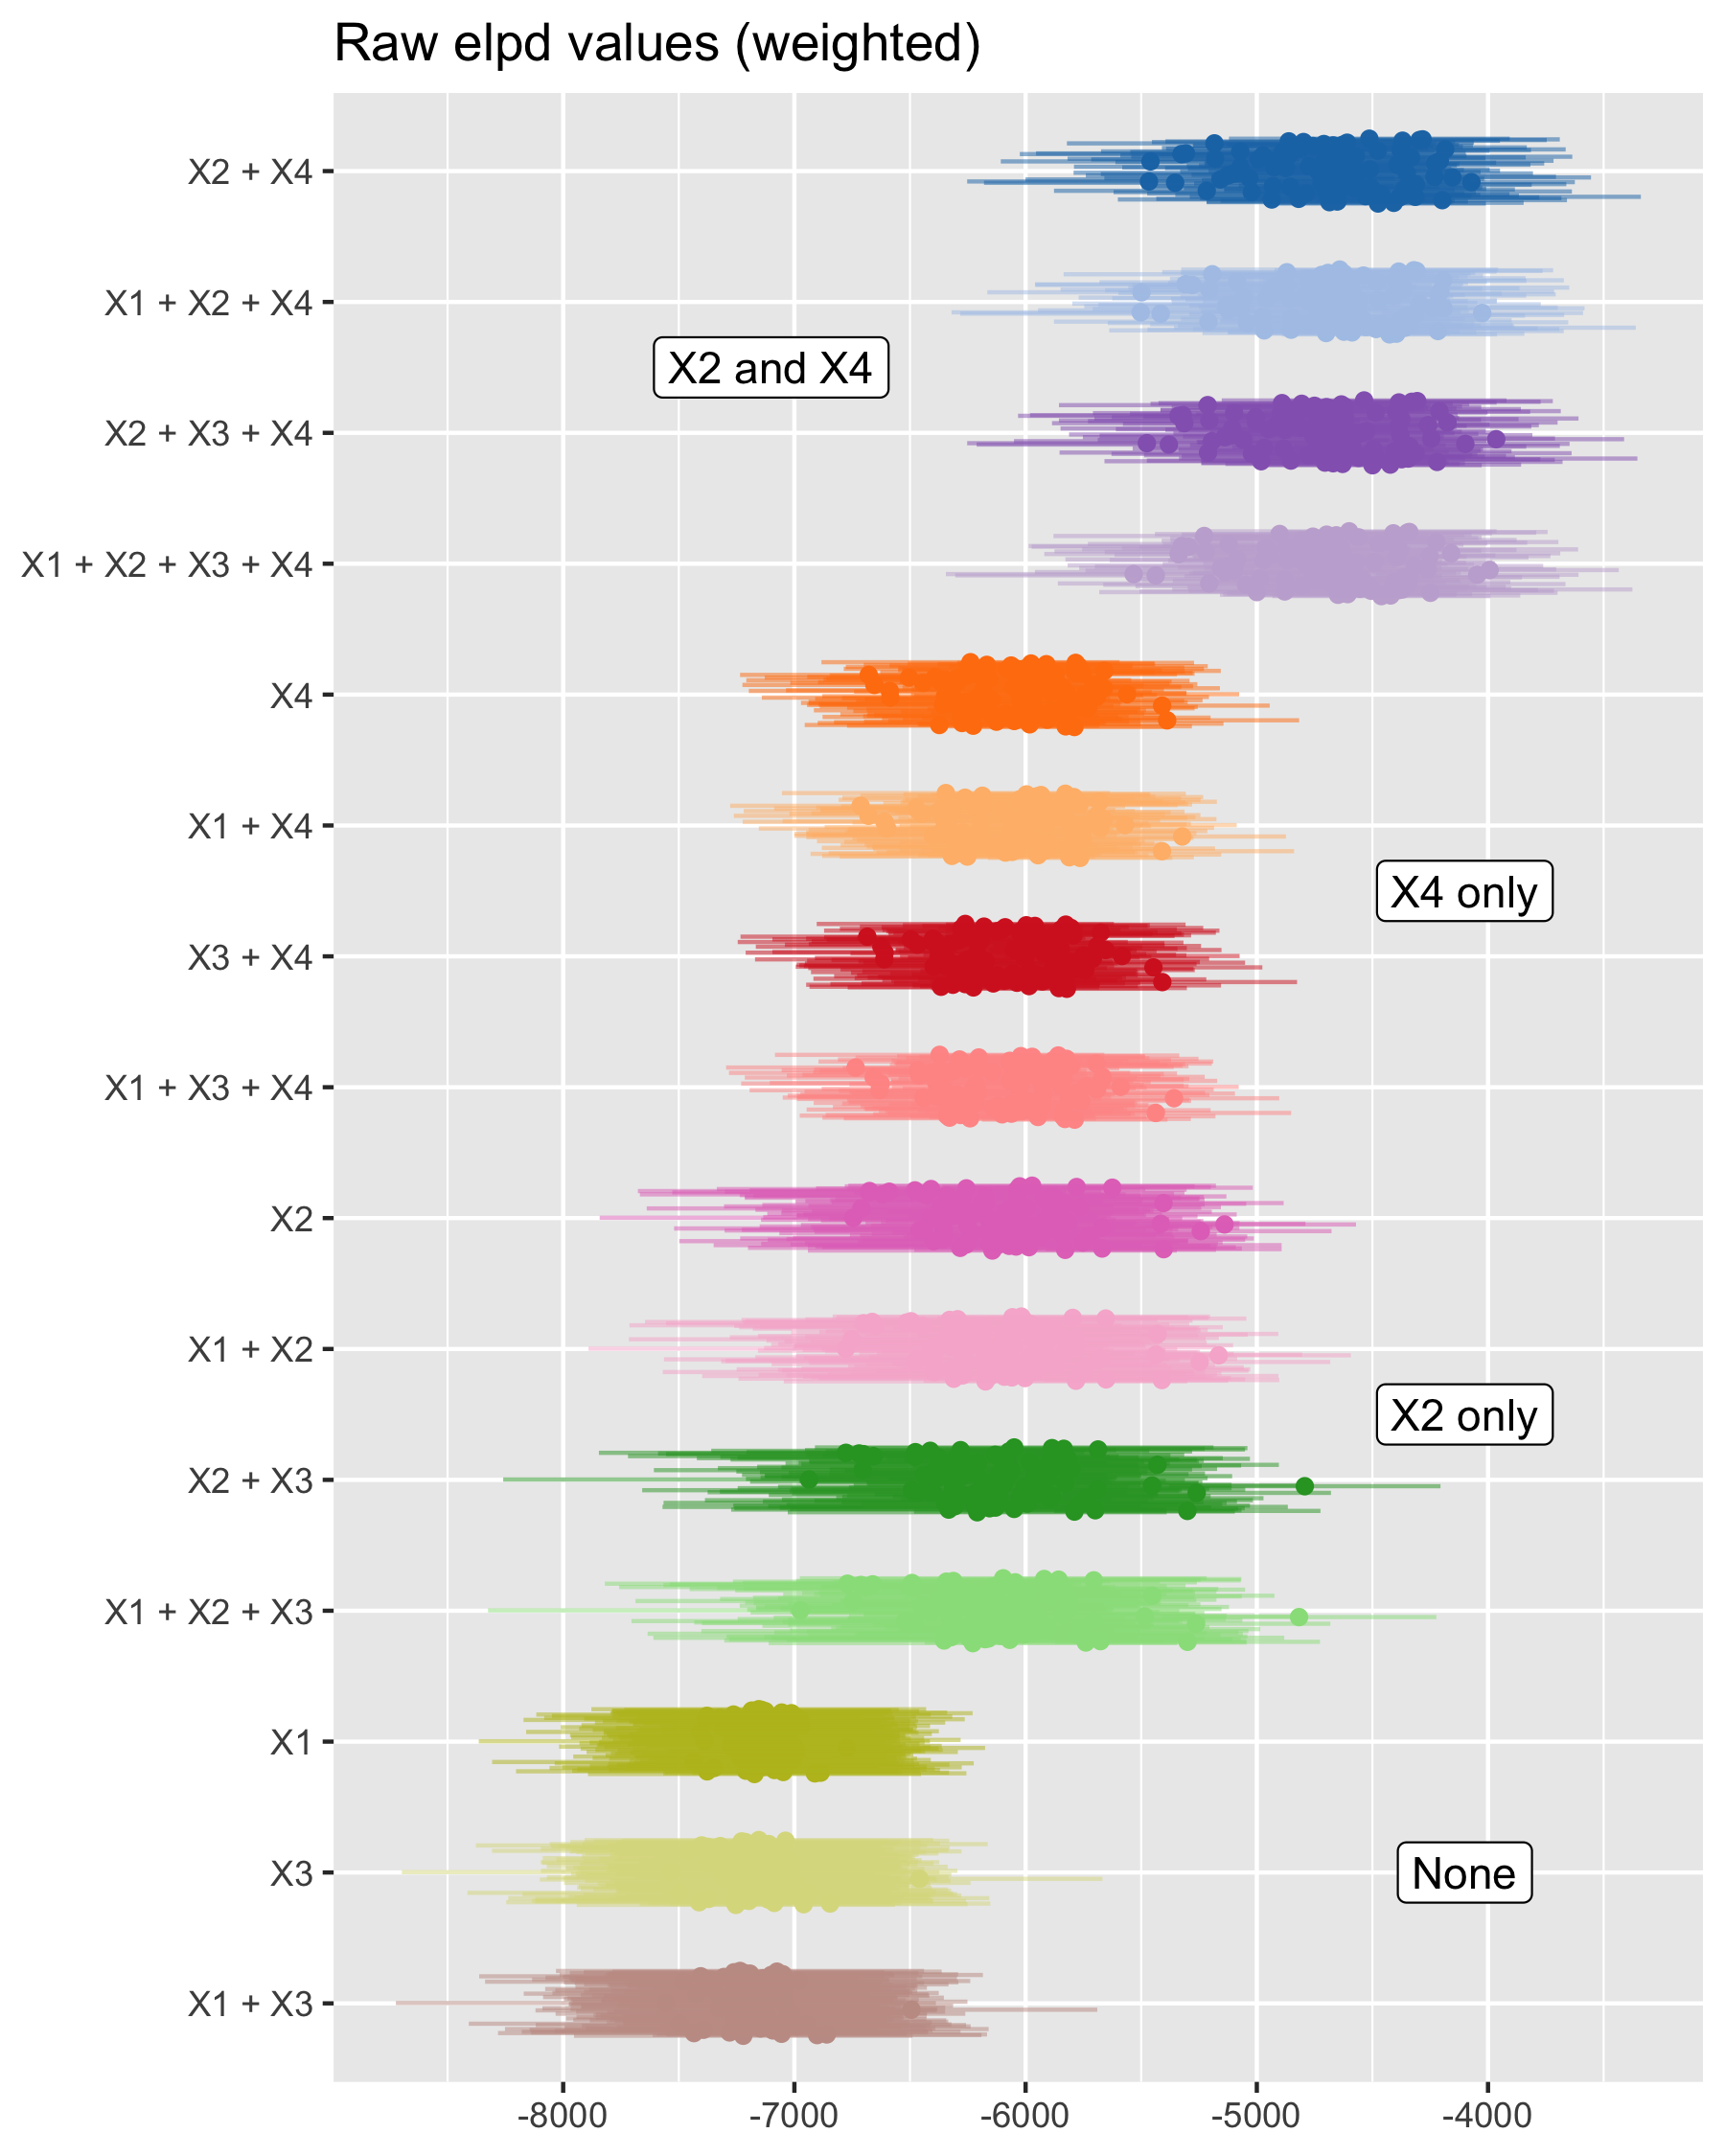
\includegraphics[width=4.6875in,height=\textheight]{images/3b/plot_loo_raw_wtd.png}

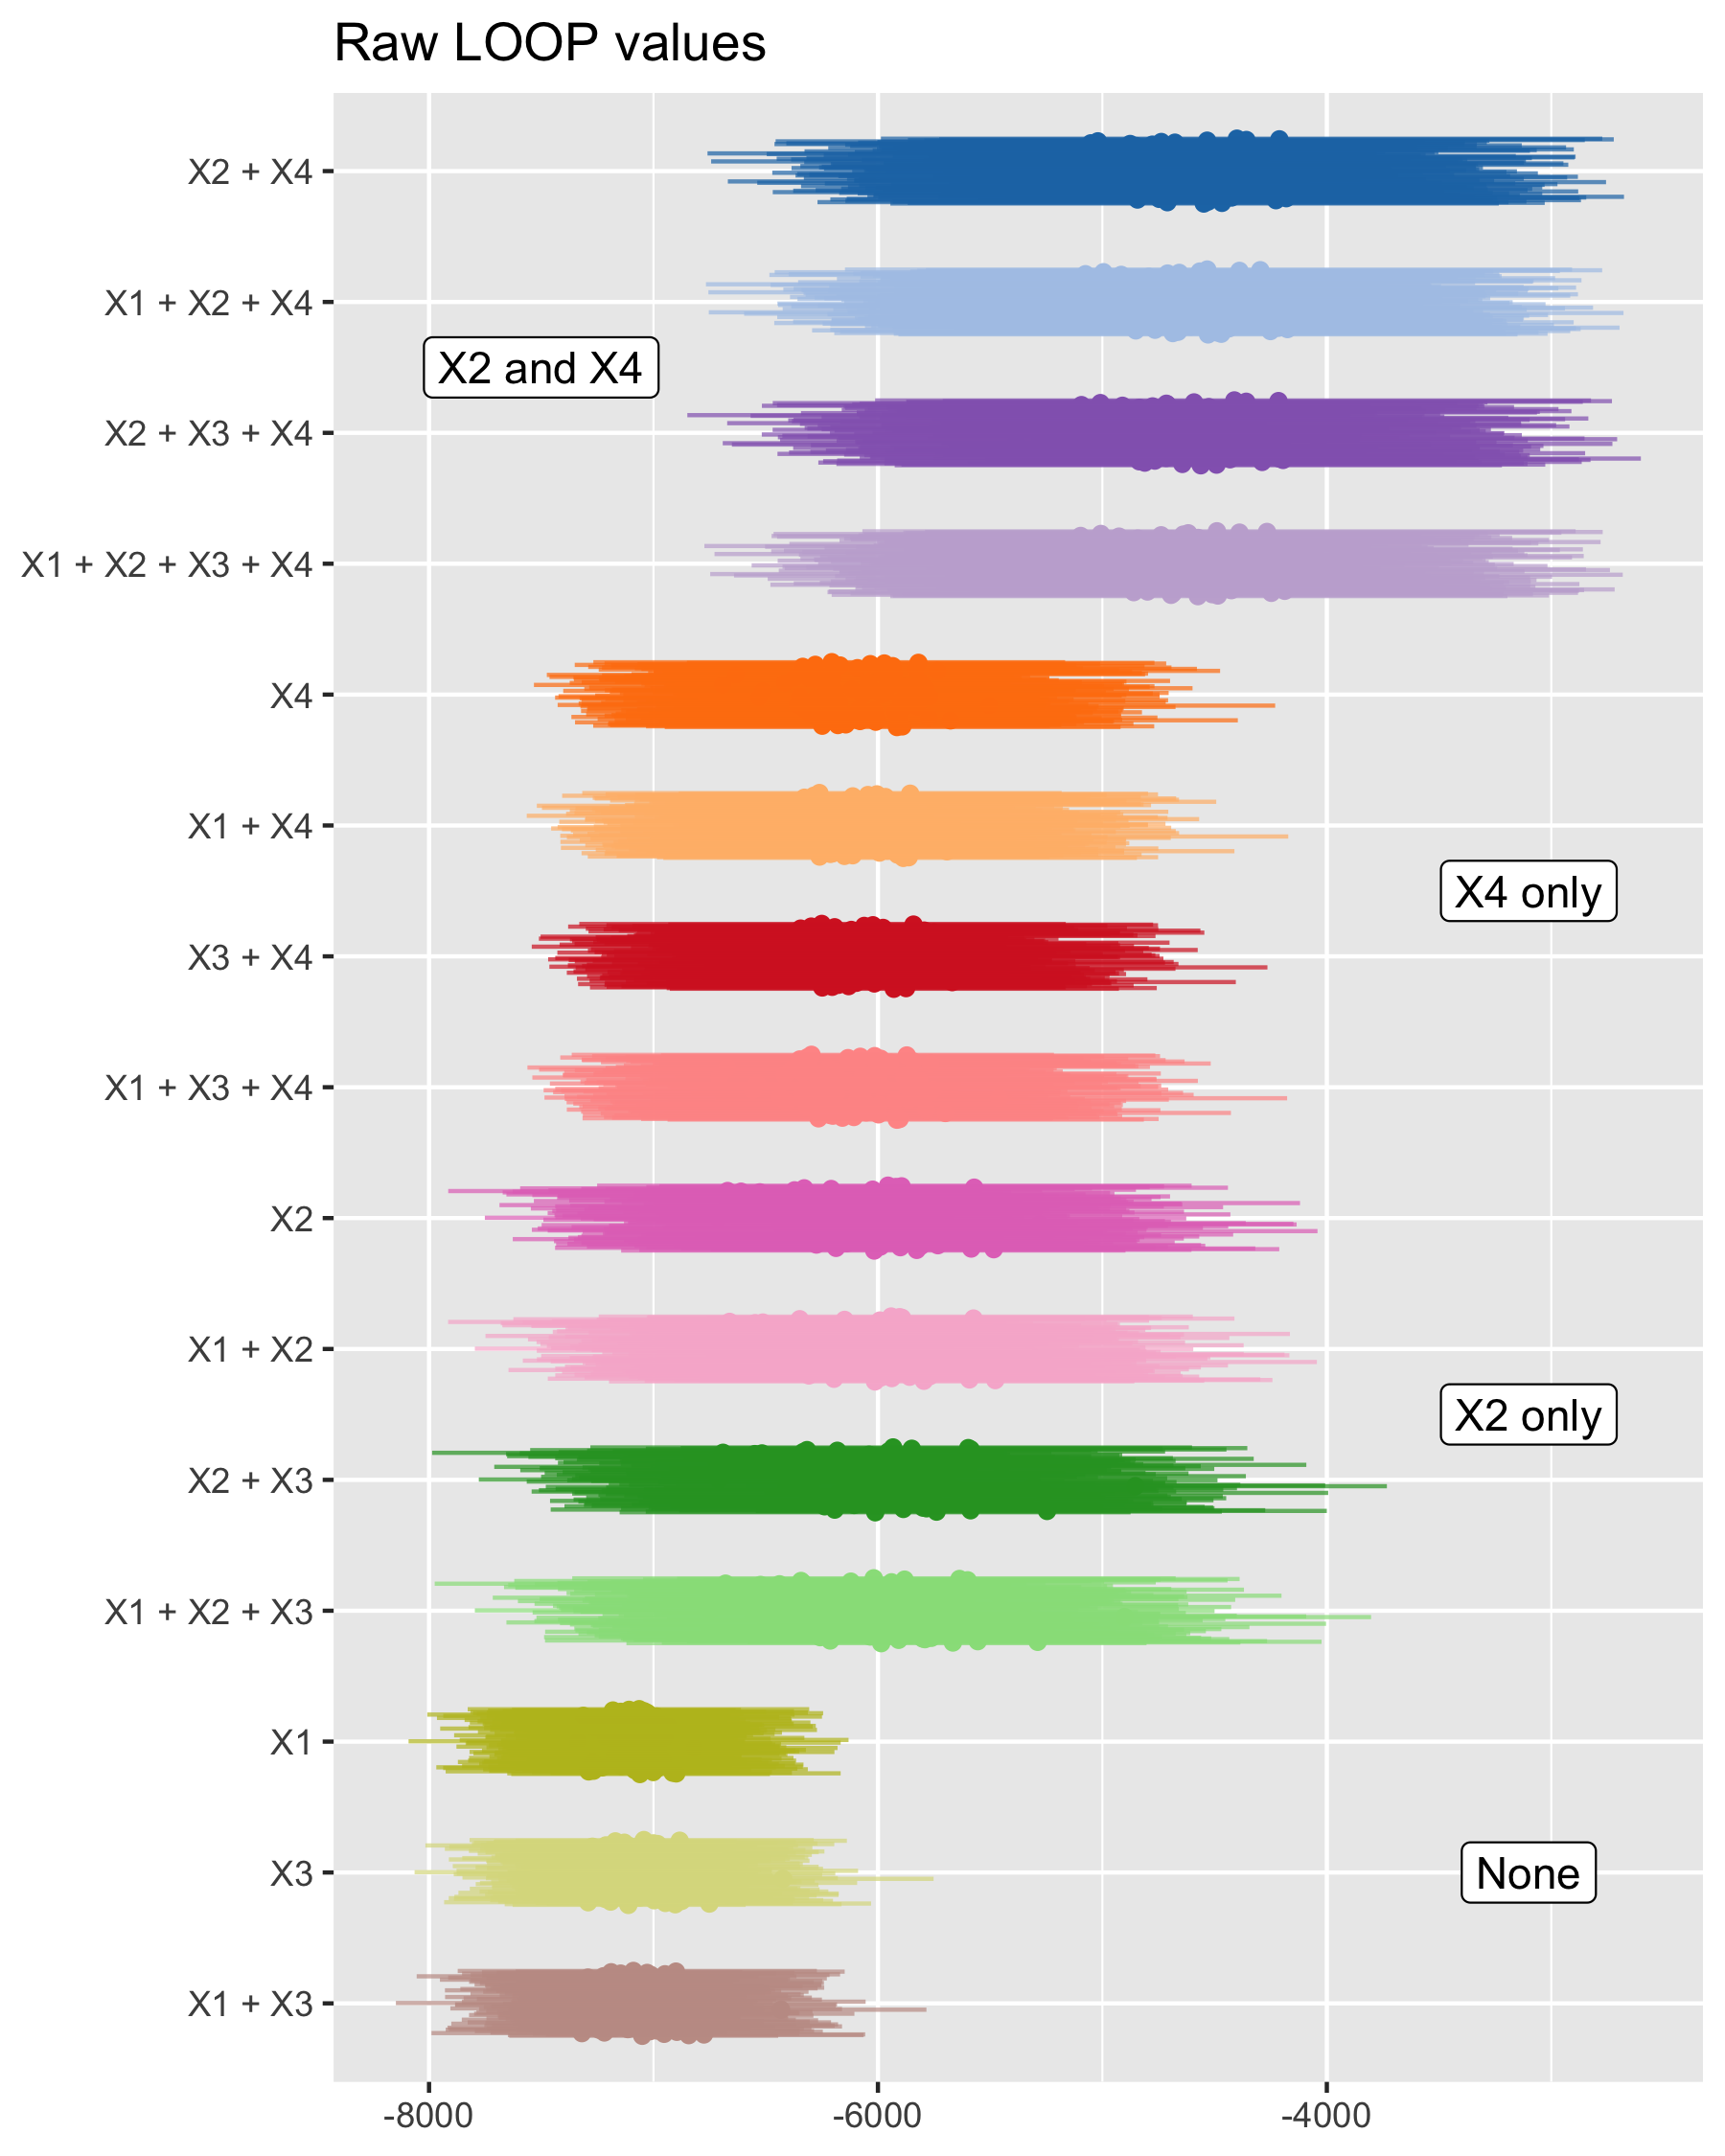
\includegraphics[width=4.6875in,height=\textheight]{images/3b/plot_loop.png}

If we look at the MRP estimates (bias), the models with both \(X_2\) and
\(X_4\) in it are distinctively less biased, as would be expected as
\(X_4\) can be seen as a bias reduction variable.

However we have higher precision (?) when we have \(X_2\) in the model.

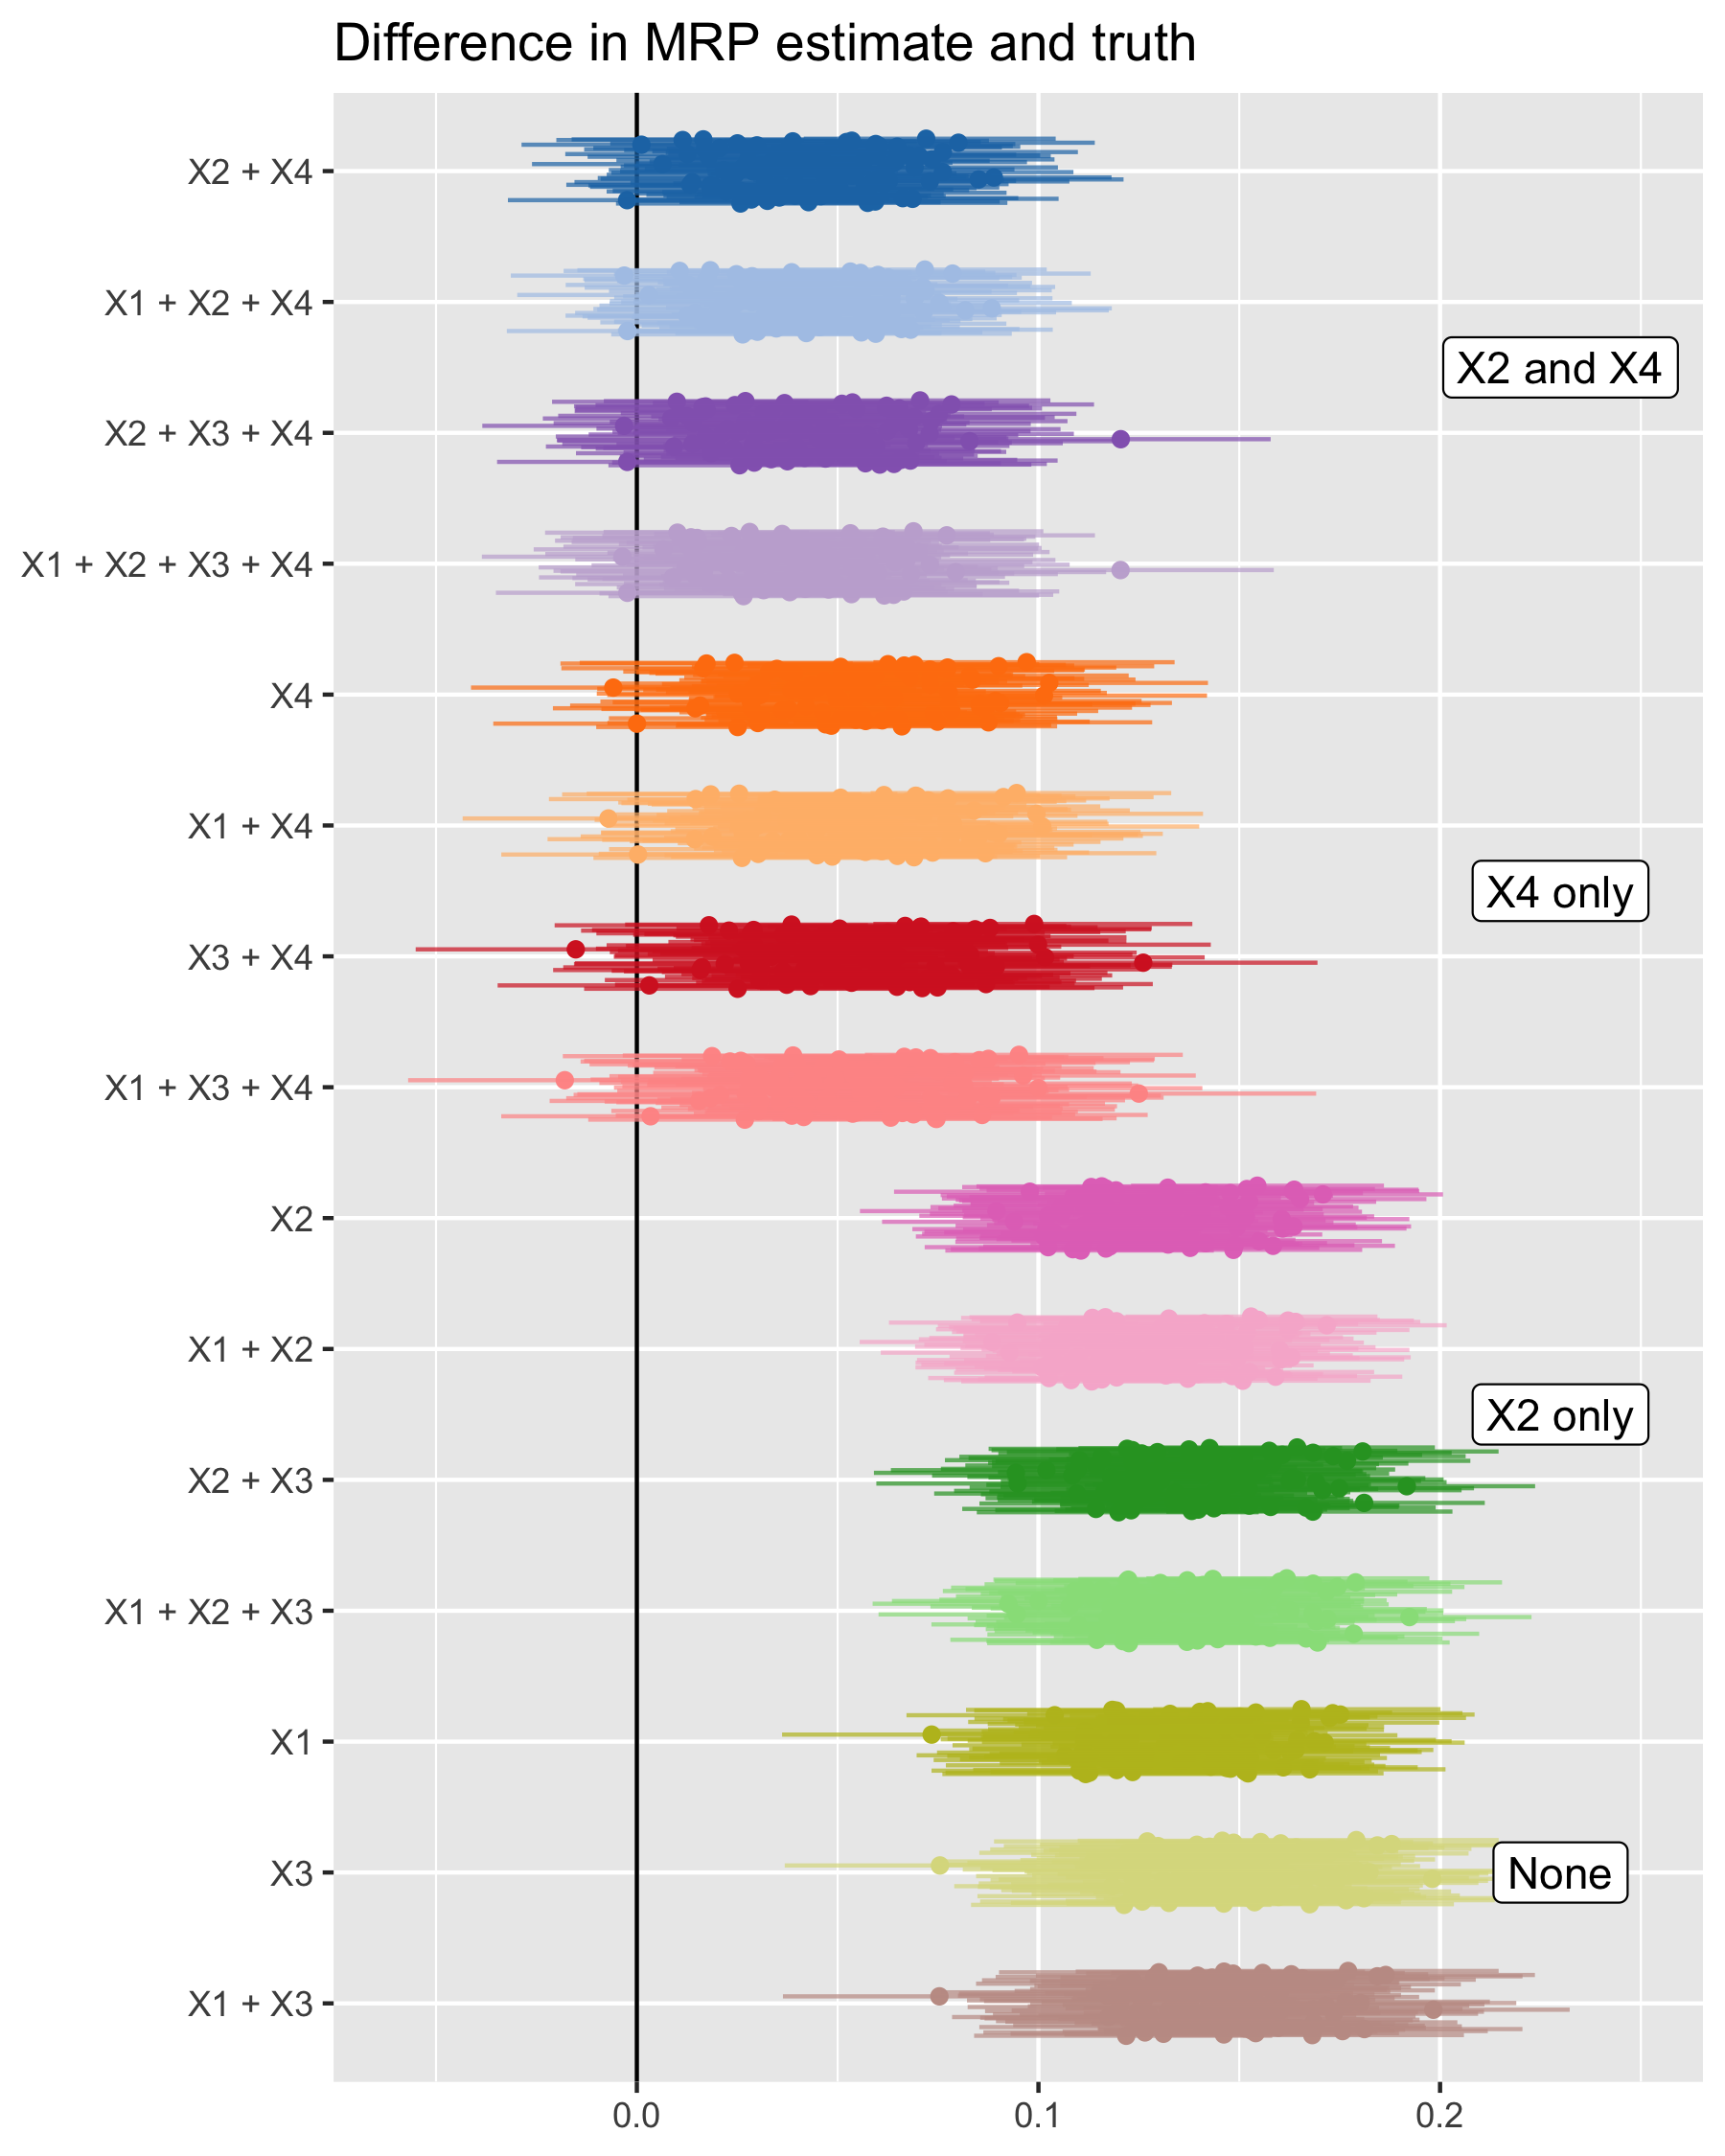
\includegraphics[width=4.6875in,height=\textheight]{images/3b/plot_mrp_truth.png}
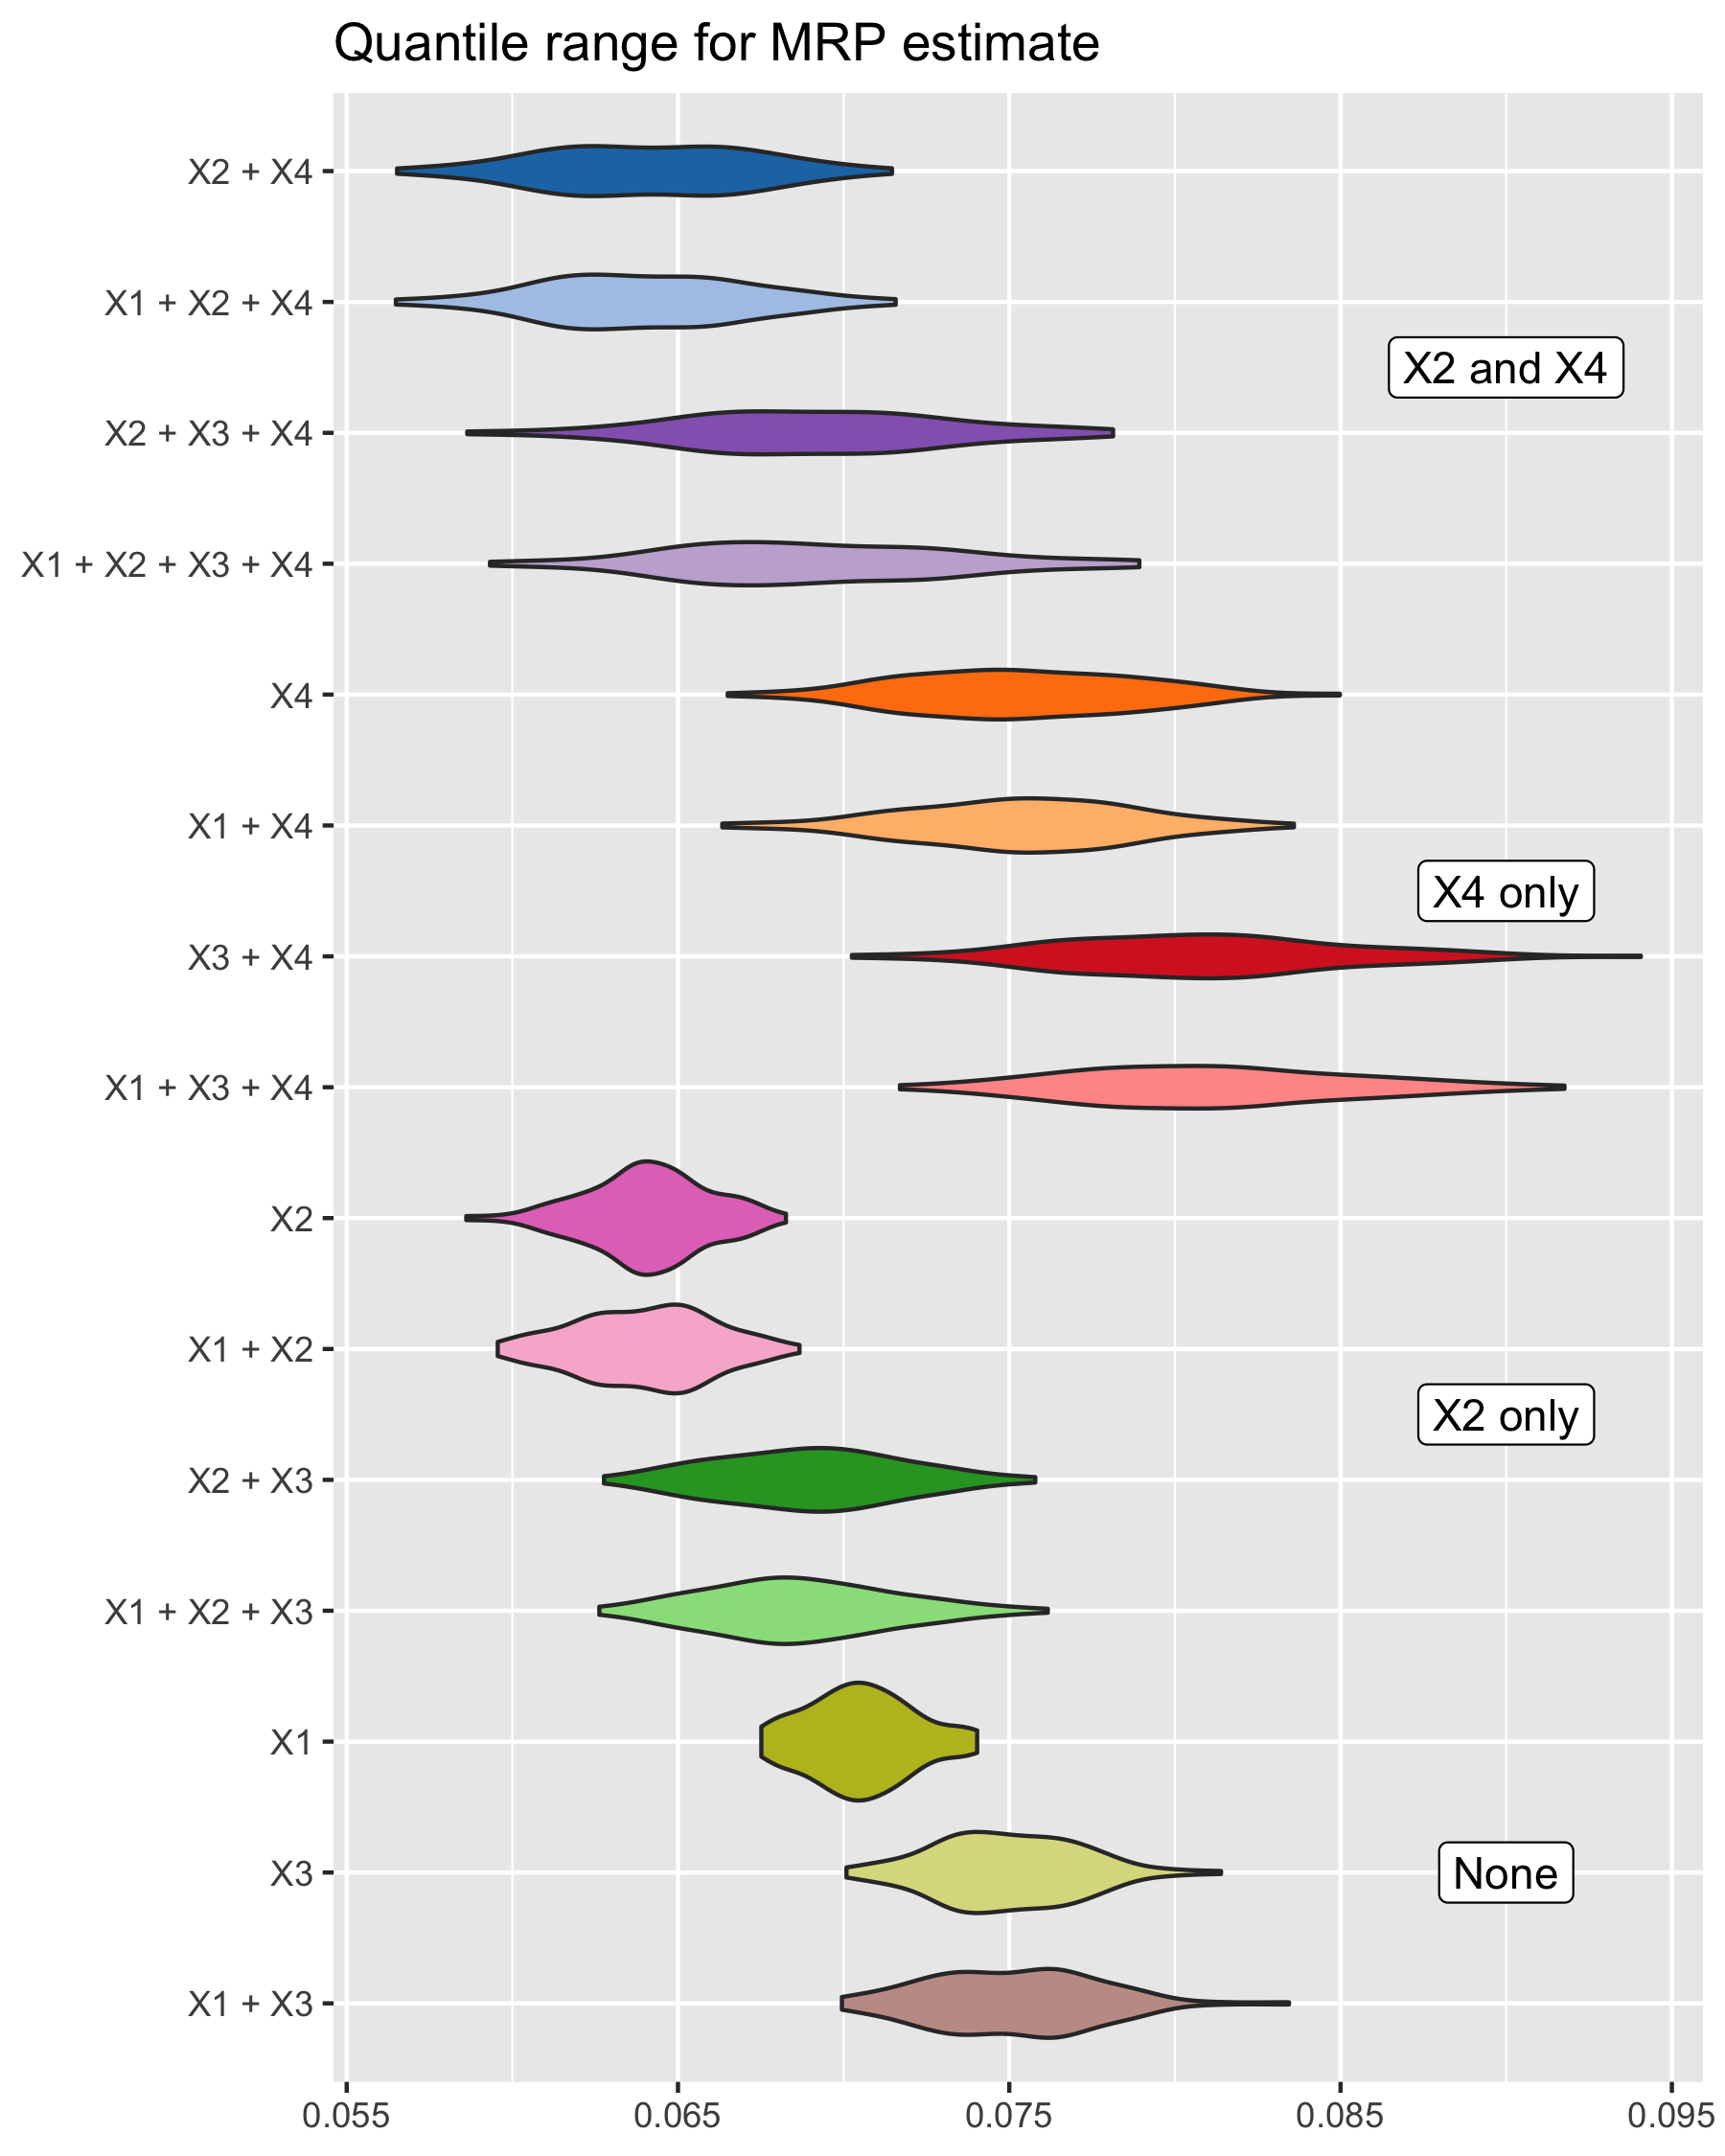
\includegraphics[width=4.6875in,height=\textheight]{images/3b/plot_mrp_qt_range.png}

\hypertarget{simulation-1}{%
\section{Simulation 1}\label{simulation-1}}

\hypertarget{finite-population-approach}{%
\subsection{Finite-population
approach}\label{finite-population-approach}}

We started with a finite population approach, using a fixed population
each time in the simulation iteration, by sampling according to the
inclusion probability. Then we calculate the \texttt{loo}'s and
\texttt{wtd\_loo}'s to compare between the models. We even tried running
different seeds for different populations.

\begin{Shaded}
\begin{Highlighting}[]
\DocumentationTok{\#\# generating 5 levels of predictors/covariates}
\NormalTok{N }\OtherTok{=} \DecValTok{10000}
\NormalTok{J }\OtherTok{=} \FunctionTok{c}\NormalTok{(}\DecValTok{5}\NormalTok{,}\DecValTok{5}\NormalTok{,}\DecValTok{5}\NormalTok{,}\DecValTok{5}\NormalTok{) }\CommentTok{\# levels for each variable}
\NormalTok{popn\_data }\OtherTok{\textless{}{-}} \FunctionTok{data.frame}\NormalTok{(}\AttributeTok{X1 =} \FunctionTok{sample}\NormalTok{(}\DecValTok{1}\SpecialCharTok{:}\NormalTok{J[}\DecValTok{1}\NormalTok{], N, }\AttributeTok{replace=} \ConstantTok{TRUE}\NormalTok{), }
                        \AttributeTok{X2 =} \FunctionTok{sample}\NormalTok{(}\DecValTok{1}\SpecialCharTok{:}\NormalTok{J[}\DecValTok{2}\NormalTok{], N, }\AttributeTok{replace=} \ConstantTok{TRUE}\NormalTok{),}
                        \AttributeTok{X3 =} \FunctionTok{sample}\NormalTok{(}\DecValTok{1}\SpecialCharTok{:}\NormalTok{J[}\DecValTok{3}\NormalTok{], N, }\AttributeTok{replace=} \ConstantTok{TRUE}\NormalTok{), }
                        \AttributeTok{X4 =} \FunctionTok{sample}\NormalTok{(}\DecValTok{1}\SpecialCharTok{:}\NormalTok{J[}\DecValTok{4}\NormalTok{], N, }\AttributeTok{replace=} \ConstantTok{TRUE}\NormalTok{))}

\DocumentationTok{\#\# generating a binary outcome }
\CommentTok{\# weakly predictive {-} 0.1 (sd), strongly predictive {-} 1 (sd)}
\FunctionTok{set.seed}\NormalTok{(}\DecValTok{748593}\NormalTok{)}
\NormalTok{popn\_data}\SpecialCharTok{$}\NormalTok{bin\_outcome }\OtherTok{\textless{}{-}} \FunctionTok{inv\_logit\_scaled}\NormalTok{(}\FunctionTok{round}\NormalTok{(}\FunctionTok{rnorm}\NormalTok{(J[}\DecValTok{1}\NormalTok{], }\AttributeTok{sd=}\FloatTok{0.1}\NormalTok{),}\DecValTok{2}\NormalTok{)[popn\_data}\SpecialCharTok{$}\NormalTok{X1] }\SpecialCharTok{+} \CommentTok{\# apply inv{-}logit for \textquotesingle{}simulated\textquotesingle{} coefficients}
                                          \FunctionTok{round}\NormalTok{(}\FunctionTok{rnorm}\NormalTok{(J[}\DecValTok{2}\NormalTok{], }\AttributeTok{sd=}\DecValTok{1}\NormalTok{),}\DecValTok{2}\NormalTok{)[popn\_data}\SpecialCharTok{$}\NormalTok{X2] }\SpecialCharTok{+}
                                          \FunctionTok{round}\NormalTok{(}\FunctionTok{rnorm}\NormalTok{(J[}\DecValTok{3}\NormalTok{], }\AttributeTok{sd=}\FloatTok{0.1}\NormalTok{),}\DecValTok{2}\NormalTok{)[popn\_data}\SpecialCharTok{$}\NormalTok{X3] }\SpecialCharTok{+}
                                          \FunctionTok{round}\NormalTok{(}\FunctionTok{rnorm}\NormalTok{(J[}\DecValTok{4}\NormalTok{], }\AttributeTok{sd=}\DecValTok{1}\NormalTok{),}\DecValTok{2}\NormalTok{)[popn\_data}\SpecialCharTok{$}\NormalTok{X4])}

\DocumentationTok{\#\# generate inclusion prob. for each individual}
\CommentTok{\# weakly predictive {-} 0.1 (sd), strongly predictive {-} 1 (sd)}
\NormalTok{popn\_data}\SpecialCharTok{$}\NormalTok{inclusion }\OtherTok{\textless{}{-}} \FunctionTok{inv\_logit\_scaled}\NormalTok{(}\FunctionTok{round}\NormalTok{(}\FunctionTok{rnorm}\NormalTok{(J[}\DecValTok{1}\NormalTok{], }\AttributeTok{sd=}\FloatTok{0.1}\NormalTok{),}\DecValTok{2}\NormalTok{)[popn\_data}\SpecialCharTok{$}\NormalTok{X1] }\SpecialCharTok{+} \CommentTok{\# apply inv{-}logit for \textquotesingle{}simulated\textquotesingle{} coefficients}
                                        \FunctionTok{round}\NormalTok{(}\FunctionTok{rnorm}\NormalTok{(J[}\DecValTok{2}\NormalTok{], }\AttributeTok{sd=}\FloatTok{0.1}\NormalTok{),}\DecValTok{2}\NormalTok{)[popn\_data}\SpecialCharTok{$}\NormalTok{X2] }\SpecialCharTok{+}
                                        \FunctionTok{round}\NormalTok{(}\FunctionTok{rnorm}\NormalTok{(J[}\DecValTok{3}\NormalTok{], }\AttributeTok{sd=}\DecValTok{1}\NormalTok{),}\DecValTok{2}\NormalTok{)[popn\_data}\SpecialCharTok{$}\NormalTok{X3] }\SpecialCharTok{+}
                                        \FunctionTok{round}\NormalTok{(}\FunctionTok{rnorm}\NormalTok{(J[}\DecValTok{4}\NormalTok{], }\AttributeTok{sd=}\DecValTok{1}\NormalTok{),}\DecValTok{2}\NormalTok{)[popn\_data}\SpecialCharTok{$}\NormalTok{X4])}
\end{Highlighting}
\end{Shaded}

We were expecting to see models with \(X_2\) and \(X_4\) getting picked
up when using \texttt{loo} and \texttt{wtd\_loo}, but we were getting
mixed results. So we moved on to a super population approach by sampling
a different population each time.

\end{document}
